% Options for packages loaded elsewhere
\PassOptionsToPackage{unicode}{hyperref}
\PassOptionsToPackage{hyphens}{url}
\PassOptionsToPackage{dvipsnames,svgnames,x11names}{xcolor}
%
\documentclass[
  letterpaper,
]{book}

\usepackage{amsmath,amssymb}
\usepackage{iftex}
\ifPDFTeX
  \usepackage[T1]{fontenc}
  \usepackage[utf8]{inputenc}
  \usepackage{textcomp} % provide euro and other symbols
\else % if luatex or xetex
  \usepackage{unicode-math}
  \defaultfontfeatures{Scale=MatchLowercase}
  \defaultfontfeatures[\rmfamily]{Ligatures=TeX,Scale=1}
\fi
\usepackage{lmodern}
\ifPDFTeX\else  
    % xetex/luatex font selection
\fi
% Use upquote if available, for straight quotes in verbatim environments
\IfFileExists{upquote.sty}{\usepackage{upquote}}{}
\IfFileExists{microtype.sty}{% use microtype if available
  \usepackage[]{microtype}
  \UseMicrotypeSet[protrusion]{basicmath} % disable protrusion for tt fonts
}{}
\makeatletter
\@ifundefined{KOMAClassName}{% if non-KOMA class
  \IfFileExists{parskip.sty}{%
    \usepackage{parskip}
  }{% else
    \setlength{\parindent}{0pt}
    \setlength{\parskip}{6pt plus 2pt minus 1pt}}
}{% if KOMA class
  \KOMAoptions{parskip=half}}
\makeatother
\usepackage{xcolor}
\usepackage[a4paper,left=1.25in,right=1.25in,top=1.00in,bottom=1.00in,textwidth=5.25in,textheight=8.75in]{geometry}
\setlength{\emergencystretch}{3em} % prevent overfull lines
\setcounter{secnumdepth}{5}
% Make \paragraph and \subparagraph free-standing
\makeatletter
\ifx\paragraph\undefined\else
  \let\oldparagraph\paragraph
  \renewcommand{\paragraph}{
    \@ifstar
      \xxxParagraphStar
      \xxxParagraphNoStar
  }
  \newcommand{\xxxParagraphStar}[1]{\oldparagraph*{#1}\mbox{}}
  \newcommand{\xxxParagraphNoStar}[1]{\oldparagraph{#1}\mbox{}}
\fi
\ifx\subparagraph\undefined\else
  \let\oldsubparagraph\subparagraph
  \renewcommand{\subparagraph}{
    \@ifstar
      \xxxSubParagraphStar
      \xxxSubParagraphNoStar
  }
  \newcommand{\xxxSubParagraphStar}[1]{\oldsubparagraph*{#1}\mbox{}}
  \newcommand{\xxxSubParagraphNoStar}[1]{\oldsubparagraph{#1}\mbox{}}
\fi
\makeatother


\providecommand{\tightlist}{%
  \setlength{\itemsep}{0pt}\setlength{\parskip}{0pt}}\usepackage{longtable,booktabs,array}
\usepackage{calc} % for calculating minipage widths
% Correct order of tables after \paragraph or \subparagraph
\usepackage{etoolbox}
\makeatletter
\patchcmd\longtable{\par}{\if@noskipsec\mbox{}\fi\par}{}{}
\makeatother
% Allow footnotes in longtable head/foot
\IfFileExists{footnotehyper.sty}{\usepackage{footnotehyper}}{\usepackage{footnote}}
\makesavenoteenv{longtable}
\usepackage{graphicx}
\makeatletter
\newsavebox\pandoc@box
\newcommand*\pandocbounded[1]{% scales image to fit in text height/width
  \sbox\pandoc@box{#1}%
  \Gscale@div\@tempa{\textheight}{\dimexpr\ht\pandoc@box+\dp\pandoc@box\relax}%
  \Gscale@div\@tempb{\linewidth}{\wd\pandoc@box}%
  \ifdim\@tempb\p@<\@tempa\p@\let\@tempa\@tempb\fi% select the smaller of both
  \ifdim\@tempa\p@<\p@\scalebox{\@tempa}{\usebox\pandoc@box}%
  \else\usebox{\pandoc@box}%
  \fi%
}
% Set default figure placement to htbp
\def\fps@figure{htbp}
\makeatother
% definitions for citeproc citations
\NewDocumentCommand\citeproctext{}{}
\NewDocumentCommand\citeproc{mm}{%
  \begingroup\def\citeproctext{#2}\cite{#1}\endgroup}
\makeatletter
 % allow citations to break across lines
 \let\@cite@ofmt\@firstofone
 % avoid brackets around text for \cite:
 \def\@biblabel#1{}
 \def\@cite#1#2{{#1\if@tempswa , #2\fi}}
\makeatother
\newlength{\cslhangindent}
\setlength{\cslhangindent}{1.5em}
\newlength{\csllabelwidth}
\setlength{\csllabelwidth}{3em}
\newenvironment{CSLReferences}[2] % #1 hanging-indent, #2 entry-spacing
 {\begin{list}{}{%
  \setlength{\itemindent}{0pt}
  \setlength{\leftmargin}{0pt}
  \setlength{\parsep}{0pt}
  % turn on hanging indent if param 1 is 1
  \ifodd #1
   \setlength{\leftmargin}{\cslhangindent}
   \setlength{\itemindent}{-1\cslhangindent}
  \fi
  % set entry spacing
  \setlength{\itemsep}{#2\baselineskip}}}
 {\end{list}}
\usepackage{calc}
\newcommand{\CSLBlock}[1]{\hfill\break\parbox[t]{\linewidth}{\strut\ignorespaces#1\strut}}
\newcommand{\CSLLeftMargin}[1]{\parbox[t]{\csllabelwidth}{\strut#1\strut}}
\newcommand{\CSLRightInline}[1]{\parbox[t]{\linewidth - \csllabelwidth}{\strut#1\strut}}
\newcommand{\CSLIndent}[1]{\hspace{\cslhangindent}#1}

\makeatletter
\@ifpackageloaded{bookmark}{}{\usepackage{bookmark}}
\makeatother
\makeatletter
\@ifpackageloaded{caption}{}{\usepackage{caption}}
\AtBeginDocument{%
\ifdefined\contentsname
  \renewcommand*\contentsname{Table of contents}
\else
  \newcommand\contentsname{Table of contents}
\fi
\ifdefined\listfigurename
  \renewcommand*\listfigurename{List of Figures}
\else
  \newcommand\listfigurename{List of Figures}
\fi
\ifdefined\listtablename
  \renewcommand*\listtablename{List of Tables}
\else
  \newcommand\listtablename{List of Tables}
\fi
\ifdefined\figurename
  \renewcommand*\figurename{Figure}
\else
  \newcommand\figurename{Figure}
\fi
\ifdefined\tablename
  \renewcommand*\tablename{Table}
\else
  \newcommand\tablename{Table}
\fi
}
\@ifpackageloaded{float}{}{\usepackage{float}}
\floatstyle{ruled}
\@ifundefined{c@chapter}{\newfloat{codelisting}{h}{lop}}{\newfloat{codelisting}{h}{lop}[chapter]}
\floatname{codelisting}{Listing}
\newcommand*\listoflistings{\listof{codelisting}{List of Listings}}
\makeatother
\makeatletter
\makeatother
\makeatletter
\@ifpackageloaded{caption}{}{\usepackage{caption}}
\@ifpackageloaded{subcaption}{}{\usepackage{subcaption}}
\makeatother

\usepackage{bookmark}

\IfFileExists{xurl.sty}{\usepackage{xurl}}{} % add URL line breaks if available
\urlstyle{same} % disable monospaced font for URLs
\hypersetup{
  pdftitle={Grundlagen des Sozialmanagements},
  colorlinks=true,
  linkcolor={Maroon},
  filecolor={Maroon},
  citecolor={Blue},
  urlcolor={Blue},
  pdfcreator={LaTeX via pandoc}}


\title{Grundlagen des Sozialmanagements}
\usepackage{etoolbox}
\makeatletter
\providecommand{\subtitle}[1]{% add subtitle to \maketitle
  \apptocmd{\@title}{\par {\large #1 \par}}{}{}
}
\makeatother
\subtitle{Begriffe - Konzepte - Ansätze}
\author{}
\date{}

\begin{document}
\frontmatter
\maketitle

\renewcommand*\contentsname{Table of contents}
{
\hypersetup{linkcolor=}
\setcounter{tocdepth}{2}
\tableofcontents
}

\mainmatter
\bookmarksetup{startatroot}

\chapter*{Über das OER Textbook}\label{uxfcber-das-oer-textbook}
\addcontentsline{toc}{chapter}{Über das OER Textbook}

\markboth{Über das OER Textbook}{Über das OER Textbook}

Dieses Open Educational Textbook ist im Rahmen des Moduls
\emph{Grundlagen des Sozialmanagements} an der
\href{https://www.fh-dresden.de}{Fachhochschule Dresden} im
Bachelorstudiengang \emph{Sozialpädagogik und -management} entstanden.
Aktuell wird es an der \href{https://www.hs-nordhausen.de}{Hochschule
Nordhausen} im Bachelorstudiengang \emph{Sozialmanagement} im
gleichnamigen Studienbereich weitergeführt. Das Textbook stellt
einerseits eine Einführung in sozial- und -betriebswirtschaftliche
Grundlagen, die Gestaltung und das Management von Organisationen in der
Sozialwirtschaft dar. Andererseits wird ausführlich auch auf das
organisationsbezogene Management in sowie die Finanzierung von
Sozialunternehmen sowie auf ausgewählte Managementkonzept in der
Sozialwirtschaft eingegangen. Das Lehrbuch entstand vor dem Hintergrund
von COVID-19 und im Bemühen um eine verstärkte Zusammenarbeit von
Studierenden, Lehrenden, Forschenden und Praktiker*innen im Sozialwesen
und Gesundheitsbereich sowie angrenzender Disziplinen und Feldern Dieses
\href{https://de.wikipedia.org/wiki/Open_Educational_Resources}{Open
Educational Resource} Textbook versteht sich als ein Wissensfundus, der
kontinuierlich ergänzt, diskutiert und weiterentwickelt wird.

\textbf{This book was last rendered on \texttt{\{r\}\ date\_rendered}.}

\section*{Lizenz}\label{lizenz}
\addcontentsline{toc}{section}{Lizenz}

\markright{Lizenz}

Dieses Buch ist kostenlos verfügbar und unter der
\href{https://creativecommons.org/licenses/by-nc-sa/4.0/}{CC BY-NC-ND
4.0 International License} lizenziert. Das bedeutet, dass das Buch
geteilt und weitergegeben werden kann, solange die Autor*innen
angemessen genannt und eventuelle geringfügige Änderungen entsprechend
gekennzeichnet werden. Geänderte Versionen, die den Inhalt remixen oder
modifizieren, dürfen jedoch nicht verbreitet werden.

\section*{Empfohlene Zitierweise (APA
7th)}\label{empfohlene-zitierweise-apa-7th}
\addcontentsline{toc}{section}{Empfohlene Zitierweise (APA 7th)}

\markright{Empfohlene Zitierweise (APA 7th)}

Arnold, M. (2020). \emph{Grundlagen des Sozialmanagements: Ein Open
Educational Textbook} (2. Aufl.). Hochschule Nordhausen.
https://doi.org/XXX.

\section*{Acknowledgement}\label{acknowledgement}
\addcontentsline{toc}{section}{Acknowledgement}

\markright{Acknowledgement}

Zur Entstehung dieses OER Textbooks haben insbesondere die folgenden
Personen beigetragen: Die Korrektur einzelner Textabschnitte haben
insbesondere Frau Sandy Albrecht, Frau Lisa Jurke, Herr Tony Krüger,
Frau Cindy Rasokat, Frau Jacqueline Seubert und Frau Tina Steinborn
unterstützt. Zu großem Dank bin ich speziell Herrn Stefan Jung
verpflichtet, der in mühseliger Kleinarbeit ein Lektorat am Manuskript
der ersten Auflage durchgeführt hat. Die Entstehung der zweiten Auflage
hat Hr. Gustavo Tadra Waldmann unterstützt.

\part{Grundlagen}

\chapter{Einführung}\label{einfuehrung}

In diesem einführenden Kapitel wird zunächst anhand einer sog.
Fachlandkarte auf das Themenfeld Sozialmanagement und Sozialwirtschaft
eingegangen. Im Anschluss folgt ein Überblick zur Geschichte und
statistischen Einordnung dieses Arbeitsfeldes bzw. gesellschaftlichen
Sektors, den wir als Sozialwirtschaft bezeichnen. Außerdem müssen
verschiedene Begriffsabgrenzungen vorgenommen werden, wie z. B. zwischen
\emph{Sozialmanagement} und \emph{Non-Profit-Management} (vgl. z. B.
Wöhrle 2017), und auch muss darauf eingegangen werden, was
Organisationen der Sozialwirtschaft von Non-Profit-Organisationen
unterscheidet.

Das Sozialmanagement lässt sich anhand einer Fachlandkarte
untergliedern. Eine Fachlandkarte wird in der Hochschuldidaktik genutzt,
um komplexe Zusammenhänge übersichtlich darzustellen und um damit
Lernenden in ein komplexes Arbeits-, Themen- und Forschungsfeld
einzuführen (vgl. z. B. Ritter-Mamczek 2016). Im Folgenden wird der
Versuch unternommen, auf einer „Schatzkarte'' die verschiedenen
Provinzen des
\href{https://de.wikipedia.org/wiki/Sozialmanagement}{Sozialmanagements}
zusammenzufassen und zu entdecken (vgl. \hyperref[figure11]{Abb. 1.1}).

\begin{figure}

\pandocbounded{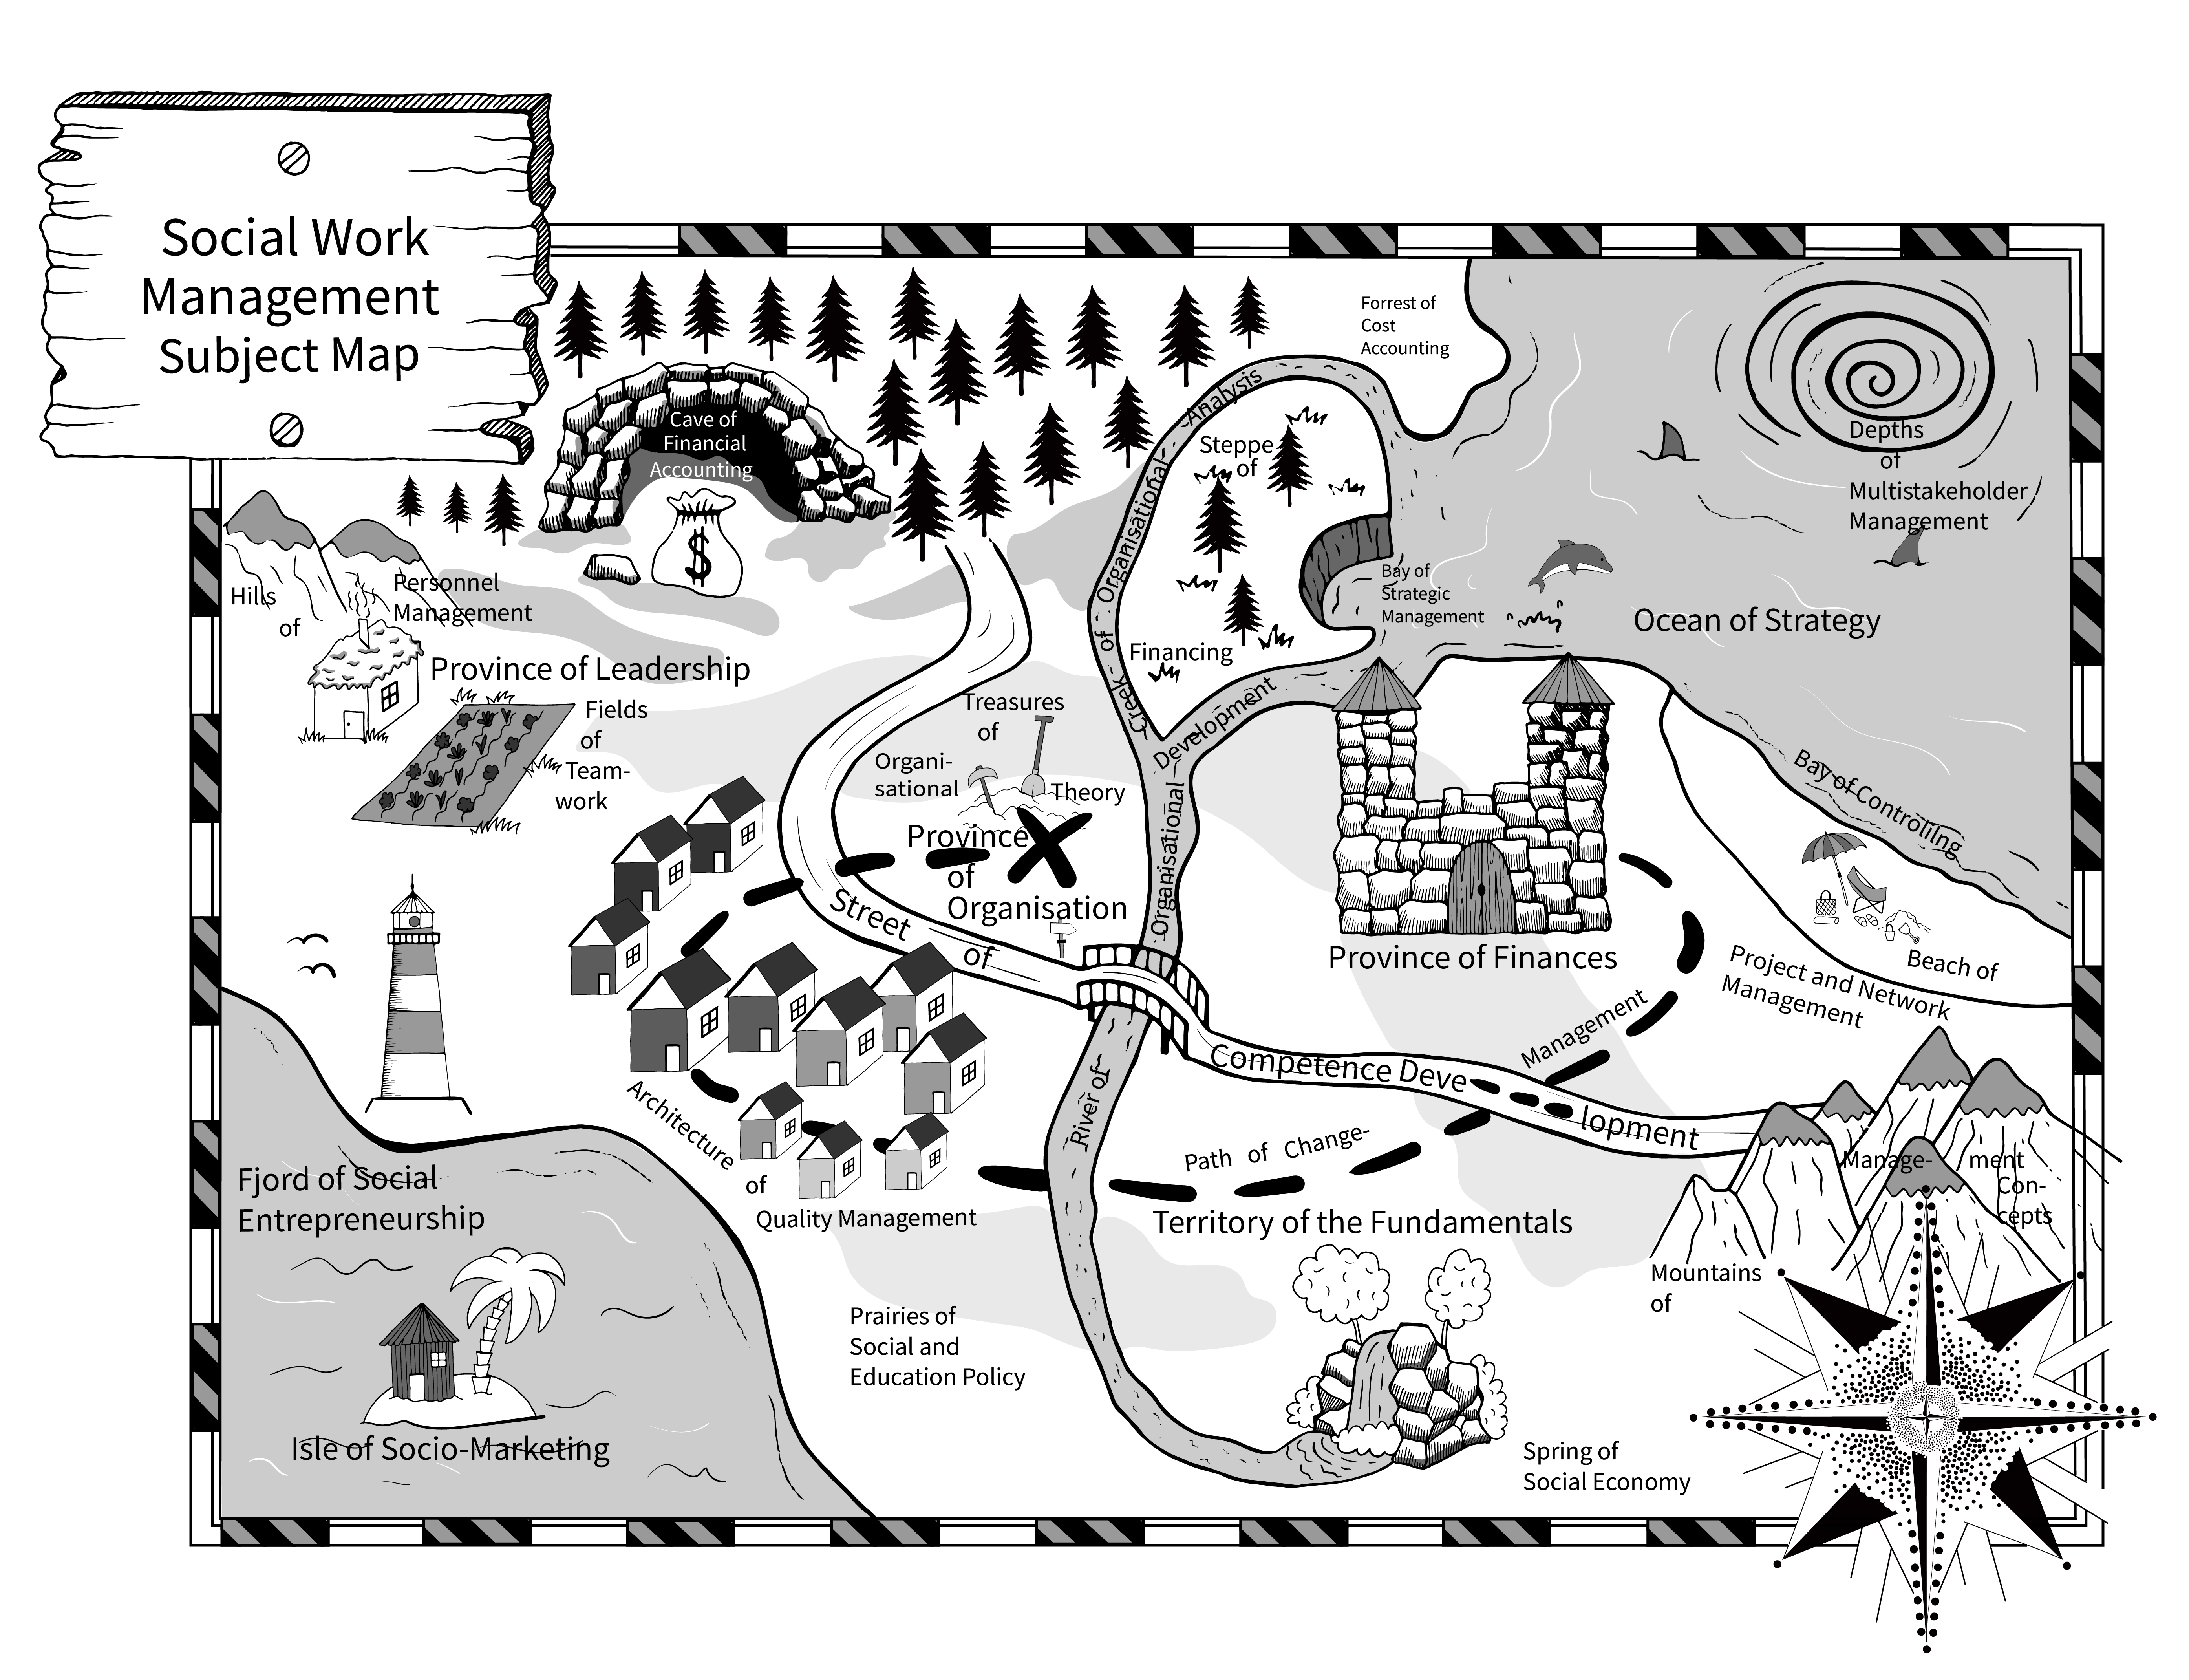
\includegraphics[keepaspectratio]{images/figure11.png}} \hfill{}

\caption{Abb. 1.1: Fachlandkarte Sozialmanagement (Arnold 2022b, CC--BY
4.0)}

\end{figure}%

Im Bild ist das \emph{Territorium der Grundlagen} zu sehen. Hier
befinden wir uns an der Quelle der Sozialwirtschaft, d.~h. es gilt die
\emph{sozialpolitischen} und \emph{bildungspolitischen
Rahmenbedingungen} und verschiedene \emph{Managementkonzepte}
kennenzulernen, wie soziale Organisation geleitet, geführt und gestaltet
werden können. Links oben im Bild ist die Höhle der
\emph{Finanzbuchhaltung} zu sehen, die sich mit der Verwaltung der
verfügbaren Finanzmittel beschäftigt. Im Wald der \emph{Kosten- und
Leistungsrechnung} können wir uns zudem einen Überblick darüber
verschaffen, wie wirtschaftlich unsere Organisation arbeitet.

Darüber hinaus ist in der Mitte des Bilds die Provinz der Organisation
zu erkennen. Man braucht ein grundlegendes Wissen über die
Organisationstheorie, z. B. darüber wie \emph{Organisationen in der
Sozialwirtschaft} aufgebaut sind, wie sie finanziert werden und wie sie
letztlich funktionieren. Dann gibt es die Provinz der Finanzen, wo es
neben der Kosten- und Leistungsrechnung und Buchführung um die Frage der
\emph{Finanzierung} geht. In diesem Zusammenhang muss ein Überblick über
die verschiedenen Finanzquellen gewonnen werden (wie z. B.
Leistungsentgelte oder Spenden). Schließlich gibt es noch am linken Rand
die Provinz des \emph{Leaderships}, wo man sich u. a. die Frage stellt,
was adäquate Mittel, Werkzeuge und Instrumente darstellen, um Führung
und Personalentwicklung innerhalb sozialer Organisationen zu gestalten.

An den Rändern der Karte sehen wir links unten das \emph{Social
Entrepreneurship} und die Insel des \emph{Sozio-Marketings}. Dort sind
alle Aufgaben- und Themenstellungen versammelt, die sich mit der
Unternehmensgründung bzw. dem Marketing beschäftigen. Darüber hinaus ist
am rechten oberen Rand der Landkarte der Ozean der Strategie abgebildet.
Im Rahmen des Sozialmanagements muss sich daher auch mit den
verschiedenen Aspekte und \emph{Grundlagen des strategischen
Managements} auseinandergesetzt werden, z. B. wie man Organisationen
langfristig leiten, gestalten und steuern kann. In der Bucht des
\emph{Controllings} kann man sich sprichwörtlich an den Strand setzen,
wo man sich das \emph{Projekt- und Netzwerkmanagement} zu Gemüte führen
kann, was natürlich auch eine wesentliche Grundkompetenz dafür
darstellt, um in sozialen Organisationen zu arbeiten.

Kurzum sind in dieser Fachlandkarte verschiedene Arbeits- und
Themenfelder zu finden, die in diesem Grundlagenlehrbuch vorgestellt und
vertieft werden. Der Fokus dieses OER Textbuchs liegt allerdings auf
einer Einführung in die sozial- und betriebswirtschaftlichen Grundlagen,
dem organisationsbezogenen Management sowie den Managementansätzen für
das Sozialmanagement liegen.\footnote{Für eine ausführliche Darstellung
  der wichtigsten Entwicklungsschritte vgl. z. B..Wöhrle, A. (2011).
  Sozialwirtschaft. In H. Thiersch, \& H. U. Otto (2011), \emph{Handbuch
  Soziale Arbeit}. \emph{Grundlagen der Sozialarbeit und
  Sozialpädagogik} (S. 1562-1570, 5. Aufl.). München: Ernst Reinhardt.
  https://doi.org/10.2378/ot4a.art145}

\section{Geschichte der Sozialwirtschaft}\label{geschichte}

\subsection[Die Anfänge der Sozialwirtschaft]{\texorpdfstring{Die
Anfänge der
Sozialwirtschaft\footnote{Für eine ausführliche Darstellung der
  wichtigsten Entwicklungsschritte vgl. z. B..Wöhrle, A. (2011).
  Sozialwirtschaft. In H. Thiersch, \& H. U. Otto (2011), \emph{Handbuch
  Soziale Arbeit}. \emph{Grundlagen der Sozialarbeit und
  Sozialpädagogik} (S. 1562-1570, 5. Aufl.). München: Ernst Reinhardt.
  https://doi.org/10.2378/ot4a.art145}}{Die Anfänge der Sozialwirtschaft}}\label{die-anfaenge-der-sozialwirtschaft}

Ein Ausflug in die Geschichte des Sozialmanagements bzw. der
Sozialwirtschaft ist notwendig, nicht nur um zu verstehen, wie sich
alles entwickelt hat, sondern auch um viele der aktuell diskutierten
Fragen rund um den Sozialstaat besser nachvollziehen zu können. Wir
beginnen in der Neuzeit, insbesondere in Frankreich, mit der ersten
Erwähnung bzw. der ersten theoretischen Auseinandersetzung mit
sozialwirtschaftlichen Grundlagen, wie z. B. der
\href{https://de.wikipedia.org/wiki/Katholische_Soziallehre}{katholischen
Soziallehre}. In den
\href{https://de.wikipedia.org/wiki/Sozialenzyklika}{päpstlichen
Sozialenzykliken} wurden bspw. Gedanken entwickelt, die später in Form
des rechtlich verbindlichen
\href{https://www.bpb.de/kurz-knapp/lexika/pocket-europa/16951/subsidiaritaetsprinzip/}{Subsidiaritätsprinzips}
weiterentwickelt wurden und mittlerweile die Rahmenbedingungen für viele
entwickelten Sozialökonomien (wie z. B. für die deutsche
\href{https://www.bpb.de/kurz-knapp/lexika/lexikon-der-wirtschaft/20642/soziale-marktwirtschaft/}{Soziale
Marktwirtschaft}) darstellen. Zur etwa gleichen Zeit ist
\href{https://de.wikipedia.org/wiki/L\%C3\%A9on_Walras}{Léon Walras} im
Rahmen seiner
\href{https://de.wikipedia.org/wiki/Walrasianisches_allgemeines_Gleichgewichtsmodell}{allgemeinen
Gleichgewichtstheorie} der Frage nachgegangen, wie Grund und Boden denn
verstaatlicht werden können. Wenn mit einer Verstaatlichung zwar Steuern
vermieden werden, so könnte seiner Meinung nach doch zumindest die
Produktion gesteigert werden. Dies soll und kann an dieser Stelle keine
vollständige Darstellung der geschichtlichen Grundlagen darstellen. Wir
wollen es bei diesen Beispielen belassen. Festzuhalten ist aber, dass
all diese verschiedene Grundlagen das „soziale Wirtschaften'' (vgl. z.
B. Beck et al. 2013) in unseren heutigen (post-)modernen Gesellschaften
zu beschreiben und zu verstehen verhelfen.

\subsection{Gründung von Genossenschaften, Diakonie und die
Bismarck'schen Gesetze}\label{gruendung}

Wenig später ist es zur Etablierung bzw. Entwicklung des
Genossenschaftswesens gekommen.
\href{https://de.wikipedia.org/wiki/Genossenschaft}{Genossenschaften}
waren ursprünglich nicht \emph{per se} als sozial-gemeinnützige
Einrichtungen ins Leben gerufen, sondern sind vielmehr dafür gegründet
worden, einen Zusammenschluss oder Verbund von Personen und
Einrichtungen zur wirtschaftlichen und/oder sozialen Förderung ihrer
Mitglieder ins Leben zu rufen, z. B. wie Raiffeisen für hilfsbedürftige
Landarbeiter oder die Volksbanken im Bankenwesen. In diesem Zusammenhang
wurden wichtige Prinzipien entwickelt, wie z. B. die
Selbstverantwortung, Selbsthilfe und Selbstverwaltung innerhalb von
Genossenschaften, die in den letzten Jahren wieder verstärkt in der
Organisationsforschung diskutiert wurden. Später kam es dann
insbesondere im Bereich der konfessionellen Trägerschaften im
\href{https://www.diakonie.de/}{Diakonie}- und
\href{https://www.caritas.de/}{Caritaswesen} zur Gründung von
Einrichtungen, die sich speziell um die Notlagen von Menschen gekümmert
haben. Beispielhaft sei hier die Gründung der ersten Stadtmission in
Deutschland von
\href{https://de.wikipedia.org/wiki/Johann_Hinrich_Wichern}{Johann
Hinrich Wichern} in Hamburg genannt. Es sollte nicht unerwähnt bleiben,
dass am Ende des 19. Jahrhunderts die
\href{https://www.bpb.de/themen/soziale-lage/rentenpolitik/289619/bismarcks-sozialgesetze/}{Bismarcksche
Sozialgesetze} eine Innovation des sozialstaatlichen Denkens darstellte
und ein wichtiges Fundament für das
\href{https://de.wikipedia.org/wiki/Sozialversicherung}{Sozialversicherungswesen}
und die Etablierung bzw. Festsetzung des
\href{https://www.bpb.de/themen/gesundheit/gesundheitspolitik/252319/das-solidarprinzip/}{Solidarprinzips}
bildete.

\subsection{Paradigmenwechsel in der Finanzierung der
Sozialwirtschaft}\label{paradigmenwechsel}

Im 20. Jahrhundert stand lange Zeit zunächst das Prinzip der
Vollkostendeckung bzw. „Selbstkostendeckung'' (Mroß 2017) im
Vordergrund, d.~h. alle Einrichtungen, die
\href{https://www.gesetze-im-internet.de/ao_1977/__52.html\#:~:text=(1)\%20Eine\%20K\%C3\%B6rperschaft\%20verfolgt\%20gemeinn\%C3\%BCtzige,sittlichem\%20Gebiet\%20selbstlos\%20zu\%20f\%C3\%B6rdern.}{gemeinnützigeZwecke}
verfolgt haben und als
\href{https://de.wikipedia.org/wiki/Leistungserbringer}{Leistungserbringer}
aufgetreten sind, haben sämtliche notwendigen finanziellen Mittel vom
Staat vollständig refinanziert bekommen. Mitte der 1970er Jahre ist aus
der Kritik am „Versorgungs- oder Wohlfahrtsstaat'' das Anliegen
entstanden, dass man insbesondere diesen Bereich der Sozialwirtschaft
und letztlich auch das Sozialmanagement stärker professionalisieren
sollte.

\subsection{Etablierung der ersten Studiengänge an
Fachhochschulen}\label{fachhochschulen}

In dieser Zeit etablierten sich die ersten Studiengänge der Sozialen
Arbeit an den Fachhochschulen, die sich vereinzelt auch mit dem Thema
auseinandergesetzt haben, wie man das Management von sozialen
Organisationen gestalten könnte. In den 1980er Jahren kam es schließlich
zu einer Etablierung von Studiengängen, die sich mit dem
Sozialmanagement oder dem Management sozialer und
Non-Profit-Einrichtungen beschäftigten. Es wurden hauptsächlich zunächst
Diplomstudiengängen und später (mit dem
\href{https://de.wikipedia.org/wiki/Bologna-Prozess}{Bologna-Reformprozess})
auch Bachelor- und Masterstudiengänge entwickelt, die sich mit dem Thema
auseinandergesetzt und versucht haben, einerseits das sozialpädagogische
und sozialarbeiterische Wissensspektrum und andererseits das
betriebswirtschaftliche Wissen zu vermitteln und weiterzuentwickeln.
Seit den 2000er Jahren haben sich dann verschiedene Studiengänge
insbesondere im Bereich des Sozialmanagements, der
Sozialwirtschaftslehre und im Non-Profit-Management etabliert, die
unterschiedliche Schwerpunktsetzungen haben und aktuelle Themen und
Aufgaben des Sozialmanagements behandeln. Heute gibt es eine kaum noch
überschaubare Vielzahl und Vielfalt an Studiengängen, die sich mit dem
Management von sozialen Organisationen und dem Management in der
Sozialwirtschaft beschäftigen (vgl. z. B. den Studienführer von
Boeßenecker and Markert 2014).

\subsection{Das neue Steuerungsmodell}\label{steuerungsmodell}

Mit dem ökonomischen Denken in den 1990er Jahren fand schließlich ein
Umdenken statt, was die Finanzierung der Sozialwirtschaft betraf. Das
ursprüngliche Kostendeckungsprinzip wurde abgelöst durch ein neues
Prinzip, nämlich das
„\href{https://de.wikipedia.org/wiki/Neues_Steuerungsmodell}{Neue
Steuerungsmodell (NSM)}``. Darauf muss später noch genauer eingegangen
werden. Nach diesem Modell soll ein Wettbewerb um die öffentlichen
Leistungen generiert werden, wobei Mittel nicht nach dem
„Gießkannenprinzip'' ausgeteilt werden. Vielmehr soll es stets
bedarfsbezogen und auch im Sinne der Sozialraumorientierung eine
Gewichtung geben, in welchen Stadtteilen beispielsweise bestimmte
Förderungen in welchem Umfang fließen.

\subsection{Soziales Unternehmertum}\label{unternehmertum}

Seit den 1960er Jahre hat man sich auch auf europäischer Ebene stärker
mit sozialpolitischen Themen auseinandersetzen müssen und eine
\href{https://www.sozialcharta.eu/}{Europäische Sozialcharta} (am 26.
Februar 1965 in Kraft getreten) entwickelt, in der festgehalten ist,
welchen Aufgabenstellungen denn ein Sozialstaat nachzukommen hat. Das
Thema des sozialen Unternehmertums bzw. Social Entrepreneurship ist dann
2011 und 2014 mit verschiedenen Initiativen auf europäischer Ebene
aufgegriffen worden (vgl. z. B. die Social Business Initiative in
European Commission 2015).

\section{Sozialwirtschaft in Deutschland und Europa}\label{deutschland}

\subsection{Gesamtwirtschaftliche Einordnung}\label{gesamtwirtschaft}

Um die Sozialwirtschaft besser in das gesamte Wirtschaftssystem
einordnen zu können, ist ein quantitativer Überblick notwendig. In einer
Untersuchung des Instituts der deutschen Wirtschaft Köln aus dem Jahr
(Institut der Deutschen Wirtschaft Köln 2004) wurden die verschiedenen
„Sozialmultis'' dargestellt (vgl. \hyperref[figure12]{Abb. 1.2}). Dabei
handelt es sich um die verschiedenen Wohlfahrtsverbände.

\begin{figure}

\pandocbounded{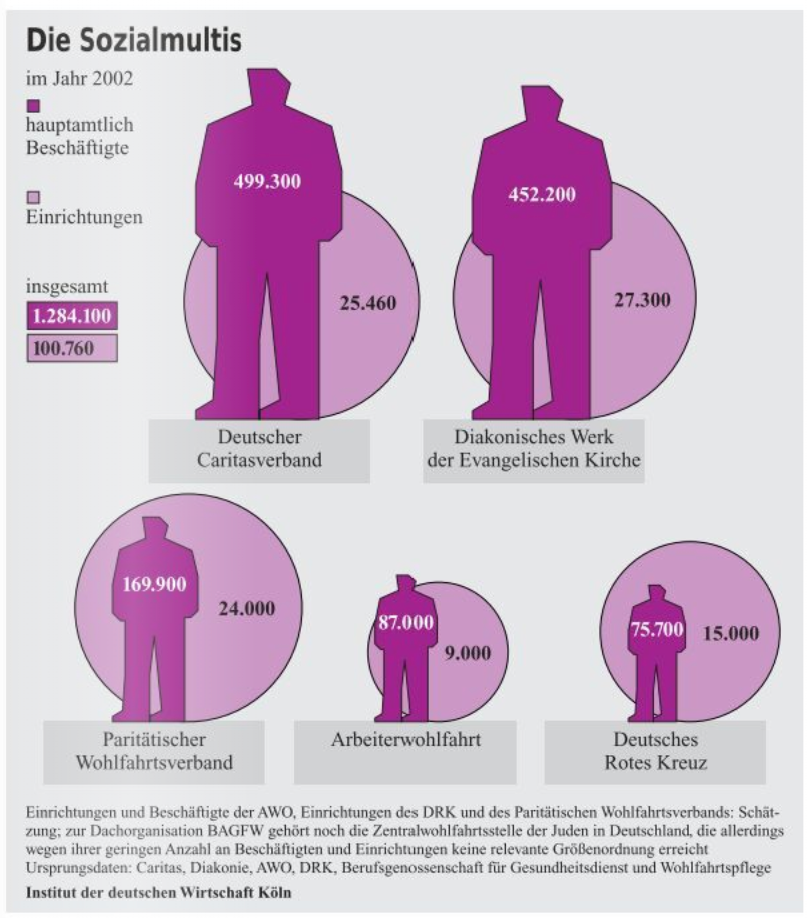
\includegraphics[keepaspectratio]{images/figure12.png}} \hfill{}

\caption{Abb. 1.2: Sozialunternehmen und Beschäftigte in der
Sozialwirtschaft (Institut der Deutschen Wirtschaft Köln 2004, S. 9,
\href{https://www.yumpu.com/de/document/view/7199735/auf-den-schultern-der-schwachen}{Link})}

\end{figure}%

Man kann deutlich erkennen, dass die konfessionellen Träger wie der
Caritasverband und auch das Diakonische Werk sowohl die meisten
Einrichtungen betreiben als auch die meisten Mitarbeitenden haben.
Darüber hinaus sind natürlich auch die anderen größeren
Wohlfahrtsverbände zu nennen, wie der Paritätische Verband, die
Arbeiterwohlfahrt und das Deutsche Rote Kreuz. Alle gemeinsam
beschäftigten im Jahre 2020 etwa rund 1,3 Millionen Menschen. Von den
Sozialmultis werden bundesweit ungefähr 100.000 Einrichtungen betrieben.
Wenn man die Träger der freien gemeinnützigen Wohlfahrtspflege
hinzunimmt, macht das ungefähr 5\% der gesamtwirtschaftlichen Leistung
aus. Wir haben ungefähr 43 Millionen Erwerbstätige in Deutschland (z. B.
Beck et al. 2013). In einem Gutachten zur Sozialwirtschaft in Sachsen
unter besonderer Berücksichtigung der Freien Wohlfahrtspflege vom
\href{https://tu-dresden.de/bu/wirtschaft/wwsprofecon/ressourcen/dateien/publikationen/Sozialwirtschaft_2011.pdf?lang=de}{Gesundheitsökonomischen
Zentrum an der TU Dresden} wurde berechnet, dass in Sachsen der Anteil
des Bereichs der „freigemeinnützigen Wohlfahrtspflege'' an der
Bruttowertschöpfung bei ungefähr 7,15\% liegt (Bundesdurchschnitt:
6,74\%) (Karmann et al. 2011).

Im Jahr 2008 gab es in Deutschland ca. 2,5 Millionen Mitarbeitende in
der Sozial- und Gesundheitswirtschaft (es wird hier der
Gesundheitsbereich hinzugerechnet) und auf europäischer Ebene rechnen
wir etwa mit 11 Millionen Mitarbeitenden in den genannten Bereichen
((Beck et al. 2013)). Wenn man dann die Wirtschaftsleistung in der
Europäischen Union betrachtet und den öffentlichen Sektor herausrechnet,
dann machen Unternehmen der Sozialwirtschaft ungefähr 10\% der
Bruttowertschöpfung aus, die eben nur der Sozialwirtschaft zugeordnet
werden können und das Gesundheitswesen ist hier in dem Fall nicht
mitgezählt (Beck et al. 2013).

\subsection{Beschäftigungszahlen}\label{beschaeftigungszahlen}

Gehen wir einmal noch auf eine andere Statistik ein, und zwar auf die
Beschäftigungszahlen in der Sozial- und Gesundheitswirtschaft. Hier sind
die Zahlen von 2014 und 2020 gegenübergestellt, die sich in den
jeweiligen Jahresberichten der Bundesagentur für Arbeit (Bundesagentur
für Arbeit Berichte 2014/2020) zum Juli des Jahres (saisonbereinigt)
finden. Im Bereich Erziehung und Unterricht sind im Jahr 2014 1.164.300
sozialversicherungspflichtig Beschäftigte angestellt gewesen. In 2020
waren bereits rund 1.347.000 Angestellte beschäftigt (15\%ige
Steigerung). In einem ähnlichen Umfang ist auch das
Beschäftigungswachstum im Bereich Gesundheitswesen auf 2.585.000
(+13,0\%) und im Bereich Heime und Sozialwesen auf 2.474.000 (+20,6\%)
gestiegen. Diese Zahlen bieten eine kurze Einordnung der
Sozialwirtschaft. Im Verhältnis dazu können wir von ungefähr 43
Millionen Erwerbstätigen in allen Branchen ausgehen.

\subsection{Finanzierungsmix für Träger der freien
Wohlfahrtspflege}\label{finanzierungsmix}

Wenn wir auf die Einnahmenseite blicken und die Frage stellen, wie denn
die freie Wohlfahrtspflege finanziert wird, dann wird deutlich, dass es
einen grundsätzlichen Mix aus unterschiedlichen Finanzierungsquellen
gibt (vgl. dazu \hyperref[figure13]{Abb. 1.3}).

\begin{figure}

\pandocbounded{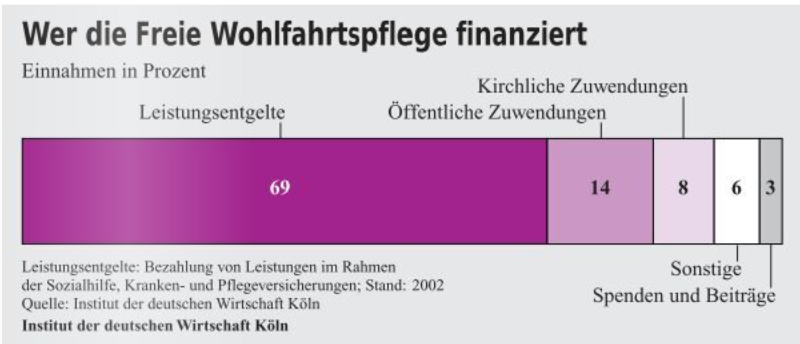
\includegraphics[keepaspectratio]{images/figure13.png}} \hfill{}

\caption{Abb. 1.3: Finanzierung der freien Wohlfahrtspflege (Institut
der Deutschen Wirtschaft Köln 2004, S. 29,
\href{https://www.yumpu.com/de/document/view/7199735/auf-den-schultern-der-schwachen}{Link})}

\end{figure}%

Nach einer Untersuchung des Instituts der deutschen Wirtschaft Köln
(Institut der Deutschen Wirtschaft Köln 2004) bestreiten zu 69\% freie
Träger ihr Einkommen aus den Leistungsentgelten. Leistungsentgelte sind
öffentliche Zuwendungen bzw. öffentliche Mittel, wie z. B. abgerechnete
Pauschalen, geleistete Fachleistungsstunden oder auch Tagessätze.
Darüber hinaus gibt es öffentliche Zuwendungen, z. B. im Rahmen von
Projekten oder institutionellen Finanzierungen. Die konfessionellen
Träger finanzieren sich teilweise noch aus kirchlichen Zuwendungen.
Schließlich gibt es noch eine Reihe von sonstigen Quellen, wie z. B.
Projektmittel, Spenden und Beiträge. Beiträge gibt es in gemeinnützigen
Einrichtungen und Organisationen, die Mitglieder haben, wie z. B.
Vereine oder Genossenschaften. Dazu zählen auch Elternbeiträge in der
Kita. Was man hier deutlich sieht -- und das ist gleichzeitig ein
Markenzeichen für die Sozialwirtschaft -- ist, dass wir es grundsätzlich
mit unterschiedlichen Finanzierungsquellen zu tun haben. Zum Erfolg
einer Einrichtung bzw. zu deren Gesamtfinanzierung reichen eben
öffentliche Mittel, die für die Finanzierung von Leistungen benötigt
werden, nicht zwingend aus. Vielmehr müssen wir uns Gedanken darüber
machen, wie wir den restlichen Betrag refinanzieren können, der nicht
auf öffentlichen, sondern dann aus privaten bzw. Eigenmitteln oder aus
Beiträgen und Spenden finanziert werden muss.

\section{Non-Profit-Organisationen}\label{npo-organisationen}

\subsection{Begriff Non-Profit-Organisationen}\label{begriffnpo}

Im Folgenden wird näher darauf eingegangen, was
Non-Profit-Organisationen ausmacht. Konkret handelt es sich dabei um
\textgreater{} „alle diejenigen Organisationen, die weder
erwerbswirtschaftliche Firmen noch öffentliche Behörden der
unmittelbaren Staats- und Kommunalverwaltung sind. NPO sind ferner jene
Organisationen, die einem gesellschaftlich als sinnvoll und notwendig
anerkannten Leistungsauftrag folgen und dabei nicht in erster Linie vom
Ziel der Gewinngenerierung geleitet werden. Nonprofit-Organisationen
werden dabei gemeinhin als Teil des sogenannten „Dritten Sektors''
verstanden, der neben bzw. zwischen den beiden idealtypischen ‚Polen'
Markt und Staat angesiedelt ist'' (Helmig 2019).

Demzufolge sind Non-Profit-Organisationen also solche Organisationen,
die nicht zum Staat und nicht zum Wirtschaftssektor gehören und
gewissermaßen den dritten Sektor in der Gesellschaft bilden. Sie
verfolgen keine Gewinnmaximierungsziele, sondern gehen einem
öffentlichen anerkannten bzw. gesetzlich geregelten Auftrag nach (siehe
\hyperref[table1]{Tab. 1}).

\begin{longtable}[]{@{}
  >{\raggedright\arraybackslash}p{(\linewidth - 2\tabcolsep) * \real{0.3913}}
  >{\raggedright\arraybackslash}p{(\linewidth - 2\tabcolsep) * \real{0.6087}}@{}}
\toprule\noalign{}
\begin{minipage}[b]{\linewidth}\raggedright
\textbf{Organisationsbereiche (nach Funktionen)}
\end{minipage} & \begin{minipage}[b]{\linewidth}\raggedright
\textbf{Typen von Organisationen}
\end{minipage} \\
\midrule\noalign{}
\endhead
\bottomrule\noalign{}
\endlastfoot
\textbf{Wirtschaftliche Organisationen} & Wirtschafts- und
Arbeitgeberverbände \\
& Gewerkschaften \\
& Berufsverbände \\
& Verbraucherorganisationen \\
\textbf{Soziokulturelle Organisationen} & Sportorganisationen \\
& Freizeitvereine \\
& Heimatvereine \\
& Diverse Kirchen, Sekten \\
& Organisationen in den Bereichen von Kunst und Kultur, von \\
& Wissenschaft und Forschung und von Bildung und Erziehung \\
& Organisationen zur Gestaltung der Lebenswelt (Wohnumfeld, \\
& Nachbarschaft etc.) \\
\textbf{Politische Organisationen} & Politische Parteien \\
& Natur- und Umweltorganisationen \\
& Politisch orientierte Organisationen \\
& Organisierte Bürgerinitiativen \\
\textbf{Karitative Organisationen} & Hilfsorganisationen für bestimmte
Bevölkerungskreise (Betagte, \\
& Behinderte, Kranke, Süchtige, Benachteiligte, Geschädigte); \\
& Wohlfahrtsverbände und deren Einrichtungen \\
& Entwicklungshilfeorganisationen \\
& Organisierte Selbsthilfegruppen mit karitativen Zwecken \\
\end{longtable}

Tab. 1: Typen privater Non-Profit-Organisationen
\phantomsection\label{table1}{Schwarz (1986), S. 7}

Auf die Frage, welche Arten von Non-Profit-Organisationen existieren,
gibt die folgende Abbildung einige Anhaltspunkte:

\begin{itemize}
\tightlist
\item
  \emph{Wirtschaftliche Organisationen}~wie z. B. Gewerkschaften,
  Arbeitgeberverbände und Verbraucherorganisationen;
\end{itemize}

\begin{itemize}
\item
  \emph{Soziokulturelle Organisationen}~wie z. B. Sportvereine,
  Organisation für Kunst und Kultur sowie wissenschaftliche
  Einrichtungen;
\item
  \emph{Politische Organisationen}~wie z. B. Parteien, Umweltbewegungen,
  Umweltverbände;
\item
  \emph{Karitative Organisationen}, die sich um die Hilfe für Menschen
  in besonderen Lebenslagen kümmern, wie z. B. Wohlfahrtsverbände und
  Entwicklungshilfeorganisationen.
\end{itemize}

Non-Profit-Organisation sind demzufolge alle Organisationen in der
Gesellschaft, die prinzipiell gemeinnützige Zwecke, aber darüber hinaus
auch wirtschaftliche Zwecke verfolgen können, aber nicht zwingend auf
eine Gewinnmaximierung aus sind. Wenn wir demgegenüber von der
Sozialwirtschaft reden, müssen wir noch eine Einschränkung vornehmen. Es
gibt zwar viele Organisationen, die hier in die Kategorie
Soziokulturelle Organisationen fallen, z. B. Organisationen zur
Förderung von Kultur oder Bildung und Erziehung. Hinzugezählt werden
müssen auch diejenigen Organisationen, die der Gestaltung des
Lebensumfeldes dienen, und auch karitative Organisationen, also alle
Wohlfahrtsverbände, Hilfsorganisationen und freigemeinnützige
Einrichtungen. Nichtsdestotrotz gibt es auch Graubereiche: Soziale
Organisationen, also spezifische Non-Profit-Organisationen; der Begriff
muss später noch näher bestimmt werden.

\subsection{Gemeinsamkeiten und Unterschiede zwischen Profit- und
Non-Profit-Organisationen}\label{vergleichnpo}

Zur genaueren Differenzierung von Non-Profit-Organisationen und
erwerbswirtschaftlichen Organisationen ist folgende
\hyperref[figure14]{Abb. 1.4} hilfreich (Schwarz 1986, S. 8).

\begin{figure}

\pandocbounded{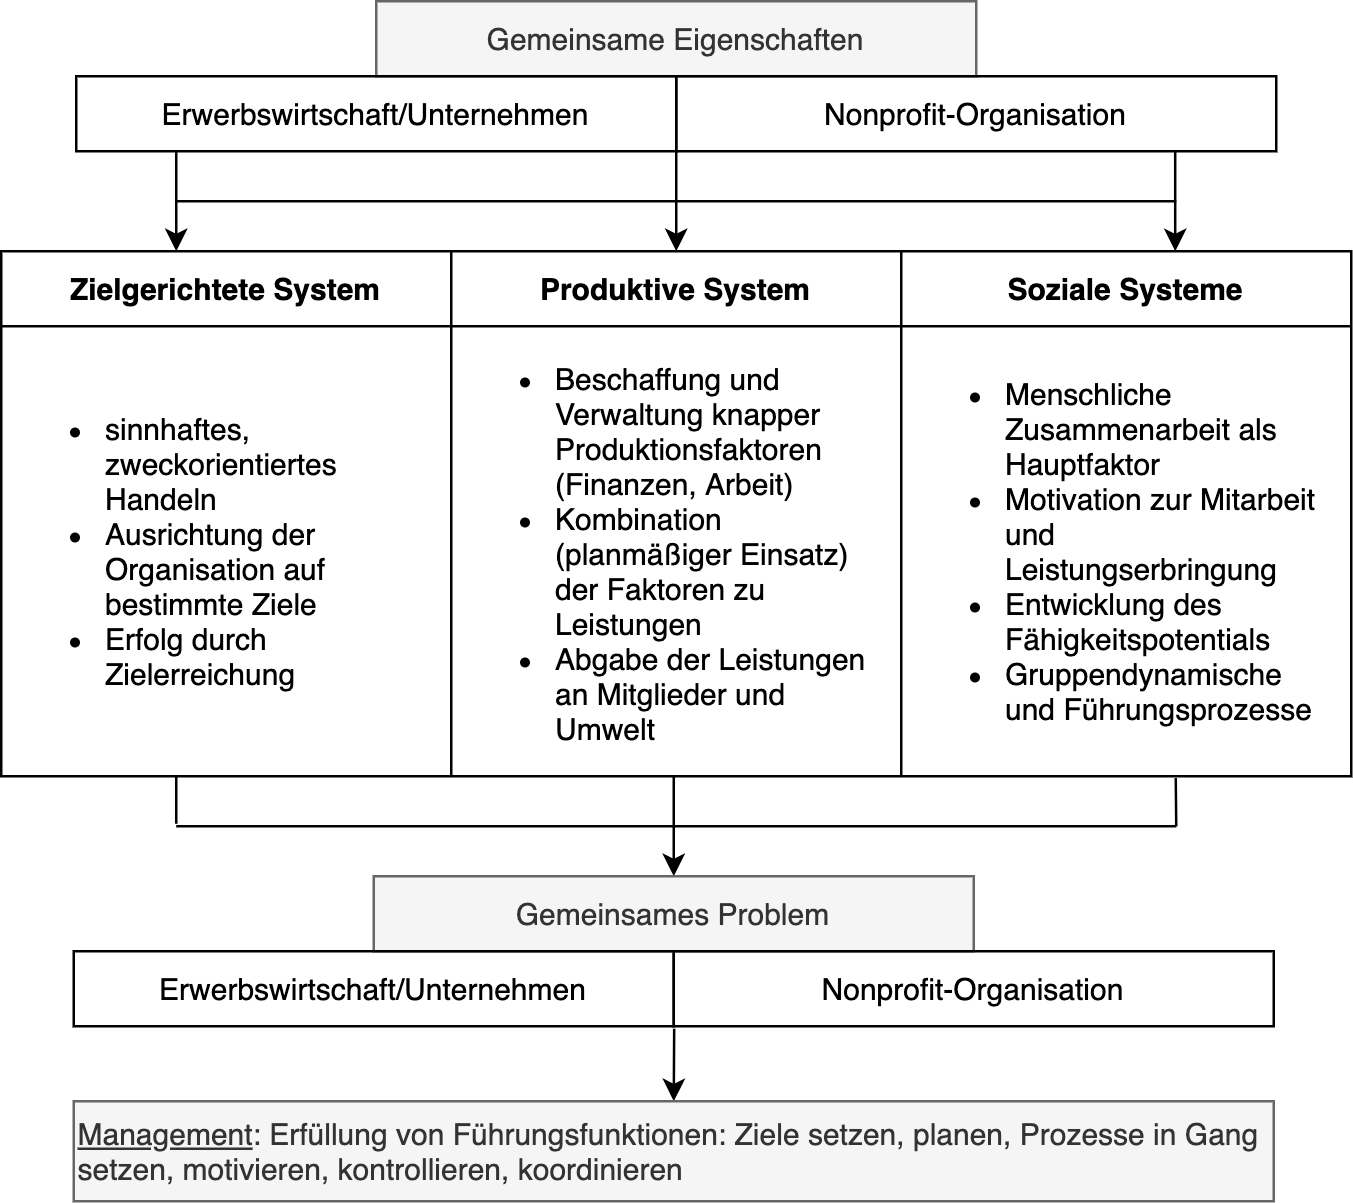
\includegraphics[keepaspectratio]{images/figure14.png}} \hfill{}

\caption{Abb. 1.4: Gemeinsamkeiten und Unterschiede zwischen NPO und
Unternehmen (nach Schwarz 1986, S. 8)}

\end{figure}%

\subsubsection{Gemeinsamkeiten}\label{npogemeinsamkeiten}

Nach Schwarz (1986) bestehen alle Organisationen, egal ob sie
erwerbswirtschaftliche (For-Profit) oder nicht-erwerbswirtschaftliche
(Non-Profit) Unternehmen darstellen, aus verschiedenen Teilsystemen.
Organisationen sind immer zugleich zielgerichtete Systeme, produktive
Systeme und soziale Systeme. Damit ist gemeint, dass jede Organisation
immer zu einem konkreten Zweck gegründet wurde, der -- wenn vorhanden --
in der Satzung bzw. im Gesellschaftervertrag der gegründeten Einrichtung
niedergeschrieben ist, und der die Grundlage bildet für das gesamte
Arbeiten in der Organisation. Darüber hinaus sind alle diese
Organisationen auch produktive Systeme, d.~h. hier geht es um die Frage,
wie ist der Personaleinsatz in der Einrichtung organisiert, welche
finanziellen Ressourcen stehen zur Verfügung, wie kann man neue
Finanzierungsquellen aufschließen und wie werden Produkte und
Dienstleistungen angeboten. Darüber hinaus sind alle Organisationen auch
soziale Systeme. Es gilt immer mit zu bedenken, wie Mitarbeitende
motiviert und dabei unterstützt werden können, ihre Kompetenzen
weiterzuentwickeln. Im Vordergrund des sozialen Systems steht also der
Faktor „Humankapital''

Alle Organisationen, sind sie denn einmal gegründet, müssen sich damit
auseinandersetzen, wie das Management ihrer Einrichtung zu funktionieren
hat, also welche Führungsprozesse zu organisieren sind, wie Ziele
gesetzt werden, wie geplant wird, wie etwa Personalplanung stattfindet
und wie Koordinierung und Organisationen im engeren Sinne in der
Einrichtung umgesetzt werden kann. All das sind Aufgaben, die jede
Einrichtung zu erfüllen hat. Kurz zusammengefasst: Auch
Non-Profit-Organisationen müssen sich mit dem Management, also mit
ökonomischen Fragestellungen auseinandersetzen und haben ähnliche
Rahmenbedingungen zu beachten wie auch erwerbswirtschaftliche
Organisationen bzw. umgekehrt.

\subsubsection{Unterschiede}\label{npounterschiede}

Und man kann neben den Gemeinsamkeiten auch verschiedene Unterschiede
herausarbeiten, auch das geht hier auf eine Untersuchung von Schwarz
Schwarz (1986) zurück (vgl. \hyperref[table2]{Tab. 2}).

\begin{longtable}[]{@{}
  >{\raggedright\arraybackslash}p{(\linewidth - 4\tabcolsep) * \real{0.2394}}
  >{\raggedright\arraybackslash}p{(\linewidth - 4\tabcolsep) * \real{0.3310}}
  >{\raggedright\arraybackslash}p{(\linewidth - 4\tabcolsep) * \real{0.4296}}@{}}
\toprule\noalign{}
\begin{minipage}[b]{\linewidth}\raggedright
\textbf{Strukturmerkmale}
\end{minipage} & \begin{minipage}[b]{\linewidth}\raggedright
\textbf{For-Profit Unternehmen}
\end{minipage} & \begin{minipage}[b]{\linewidth}\raggedright
\textbf{Non-Profit Organisationen}
\end{minipage} \\
\midrule\noalign{}
\endhead
\bottomrule\noalign{}
\endlastfoot
\textbf{Hauptzweck} & Erwirtschaftung eines möglichst hohen Ertrags auf
das investierte Kapital für Eigentümer (Formalziele: Gewinn und
Rentabilität) -- Erwerbswirtschaft & Erbringung von Leistungen für
bestimmten Personenkreis in der Sozial- und Gesundheitswirtschaft
(Sachziel: satzungsgemäße Zwecke) -- Bedarfswirtschaft \\
\textbf{Adressaten und Marktbeziehung} & Deckung des Fremdbedarfs von
Nachfrage durch Angebot auf Märkten & Deckung des Eigenbedarfs von
Mitgliedern, Klienten etc. und des gesellschaftlichen Bedarfs
(Identitätsprinzip: Mitglied = Kunde) \\
\textbf{Steuerungsprinzipien} & Marktorientierung, Ausrichtung an
Kunden- und Wettbewerberverhalten & Marktsteuerung teils nicht existent,
teils sekundär; Mitglieder bestimmen demokratisch (direkt) oder durch
indirektes Verhalten über Leistung (Versorgungs- und
Bedarfsorientierung) \\
\textbf{Güter und Dienstleistungen} & Nur private marktfähige
Individualgüter, die ausschließlich vom einzelnen Käufer genutzt werden
können & Kollektivgüter, die einer ganzen Gruppe zugutekommen, auch
denjenigen, die nicht dafür zahlen können; hauptsächlich
Dienstleistungen \\
\textbf{Finanzmittel} & Kapitalanlagen und Umsatzerlöse &
Mitgliedsbeiträge, Leistungsentgelte, Spenden, Steuervergünstigungen
etc. \\
\end{longtable}

Tab. 2: Unterscheidung von Unternehmen der Erwerbswirtschaft und
Non-Profit-Organisationen \phantomsection\label{table2}{Schwarz (1986)}

Der Hauptzweck von Non-Profit-Organisationen ist insbesondere, dass hier
Leistungen für einen ganz bestimmten Personenkreis der Sozial- und
Gesundheitswirtschaft erbracht werden. Man spricht in diesem
Zusammenhang auch von einer Bedarfswirtschaft, d.~h. es wird immer
anhand von gesetzlichen Rahmenbedingungen bzw. den Bedürfnissen der
jeweiligen Zielgruppe aus geplant, während die Erwerbswirtschaft stärker
den Blick darauf richtet, das eingesetzte Kapital und den Ertrag zu
steigern. In der Erwerbswirtschaft steht daher der Gewinn und die
Rentabilität im Blick als Formalziele im Vordergrund. Profitorientierte
Organisationen haben die Nachfrage und das Angebot auf Märkten im Blick,
während Non-Profit-Organisationen den Eigenbedarf ihrer Mitglieder,
Klient*innen bzw. allgemein den gesellschaftlichen Bedarf
berücksichtigen müssen. Man spricht in letzterem Fall von sozialen
Märkten bzw. vom Gesundheitsmarkt, was einen abgegrenzten Bereich
darstellt.

Ebenso unterscheiden sich die Steuerungsprinzipien zwischen Profit- und
Non-Profit-Bereich. Die Erwerbswirtschaft orientiert sich am Markt und
richtet ihre Produkte und Dienstleistungen an den möglichen
Entwicklungen im Markt aus. Dabei müssen Wettbewerb, Kundenorientierung
und das Verhalten der Wettbewerber und Kunden ständig analysiert werden,
während es bei den Non-Profit-Organisationen eher darum geht, dass
Mitglieder mitbestimmen können, wie die Einrichtungen sich entwickeln
und auch, dass insbesondere die Perspektiven der Klient*innen in den
Mittelpunkt geschoben werden. Die angebotenen Güter und Dienstleistungen
unterscheiden sich zwischen Profit- und Non-Profit-Organisationen.
Profitorientierte Organisationen setzen die auf Märkten gehandelte
Individualgüter ab. Es kann natürlich auch Produktionsgüter geben.
Schwarz (1986) sagt, dass Non-Profit-Organisationen tendenziell eher
Kollektivgüter produzieren, mit anderen Worten also soziale
Dienstleistungen anbieten. Auch hinsichtlich der Finanzmittel gibt es
Unterschiede. Profitorientierte Organisation können beispielsweise Geld
am Kapitalmarkt anlegen und finanzieren sich aus Umsatzerlösen. Bei den
Non-Profit-Organisationen existieren verschiedene Einnahmequellen, wie
z. B. Leistungsentgelte, öffentliche Zuwendungen, Mitgliederbeiträge
oder Spenden.\\
\strut \\
Abschließend muss der hier nach Schwarz (1986) vorgestellte Ansatz noch
einmal kritisch betrachtet werden. Diese Übersicht ist natürlich eine
Vereinfachung, um wesentliche Unterschiede zwischen diesen Typen von
Unternehmen herauszuarbeiten. Die Übersicht stammt auch aus den 1980er
Jahren und wurde in verschiedenen Lehrbüchern immer wieder reproduziert.
Daher nehmen wir hier auch Bezug darauf. Beachtet werden muss
allerdings, dass sich die Grenzen zwischen Profit- und
Non-Profit-Organisationen über die letzten Jahre hinweg verschoben
haben. Selbstverständlich gibt es auch Grenzbereiche bzw. eine Grauzone.
So gibt es natürlich auch viele Non-Profit-Organisationen, die neben
ihrer gemeinnützigen Arbeit auch noch einen wirtschaftlichen
Geschäftsbetrieb besitzen und dort eine Gewinnmaximierung verfolgen
können. Genauso gibt es auch For-Profit-Organisationen, die im Bereich
der Sozialwirtschaft tätig sind, wie z. B. Pflegeeinrichtungen für
einkommensstärkere Bevölkerungsgruppen, die durch Eigen- bzw.
Selbstbeiträge andere und umfangreichere Dienstleistungen (über den
gesetzlichen Anspruch hinaus) beanspruchen können. All das sind
sozusagen auch erwerbswirtschaftliche Sichtweisen bzw. Elemente, die
auch in der Sozialwirtschaft immer mehr an Bedeutung gewinnen. Das
bringt uns zu dem Punkt, dass wir bei der Unterscheidung von For-Profit-
und Non-Profit-Organisationen von einem breiten Spektrum ausgehen
müssen. Auf der anderen Seite des Spektrums stehen idealtypisch die
For-Profit-Organisationen, auf der anderen Seite die
Non-Profit-Organisationen. In der Realität befinden wir uns
möglicherweise immer zwischen diesen verschiedenen Idealtypen. Im
Folgenden werden wir demnach Organisationen in den Blick nehmen, die
„tendenziell'' Non-Profit-Organisationen darstellen und die im erwähnten
Spannungsfeld zwischen diesen beiden Polen stehen.

\section{Begriff Soziale
Organisation}\label{begriff-soziale-organisation}

In Abgrenzung zum Begriff Non-Profit-Organisation wird nunmehr noch eine
Abgrenzung zu dem der „Sozialen Organisation'' notwendig. Die Merkmale
von Sozialen Organisationen lassen sich wie in der folgenden Liste
versuchen festzumachen:

\begin{itemize}
\item
  Soziale Einrichtungen sind insbesondere Unternehmen, die
  Sozialdienstleistungen erbringen und/oder Güter und Dienstleistungen
  für besonders schutzbedürftige Bevölkerungsgruppen und entsprechend
  gesetzlicher Aufträge (z. B. Erziehung, Betreuung, Lernen) anbieten.
  Diese Sozialunternehmen streben im Rahmen der Produktion von Waren
  bzw. bei der Erbringung von Dienstleistungen ein soziales Ziel an.
\item
  Sie zielen im Sinne der Gemeinnützigkeit auf eine Bedarfs- und
  Kostendeckung anstatt auf Gewinnmaximierung. Nichtsdestotrotz müssen
  auch soziale Einrichtungen Gewinne erwirtschaften, d.~h. am Ende des
  Jahres muss etwas überbleiben. Dieser Überschuss muss allerdings
  wieder dem Einrichtungszweck zugutekommen. Die Gemeinnützigkeit ist in
  der Abgabenordnung geregelt, nach der der Gesetzgeber den als
  gemeinnützig anerkannten Einrichtungen Steuerermäßigungen/-befreiungen
  einräumt, wie z. B. für Ertragsteuern, Umsatzsteuer etc.
\item
  Sie offerieren „soziale personenbezogene Dienstleistungen'' (Klatetzki
  2010), die sich aus gesetzlich normierten Aufträgen (z. B.
  \href{https://www.bpb.de/kurz-knapp/lexika/politiklexikon/18231/sozialgesetzbuch-sgb/}{SGB})
  ergeben. Eine Besonderheit dieser Art von Dienstleistungen ist es,
  dass diese in dem Moment, wenn sie angeboten werden, bereits
  verbraucht werden, weil hier Produktion und Konsumption gewissermaßen
  zusammenfallen. Soziale personenbezogene Dienstleistungen können nur
  schwer standardisiert werden. Anders als bei einem Werkstück, was man
  in eine Maschine einspannt und ausmessen kann, sind hier
  professionelle Normen, Haltungen und Ansprüche gemeint, die wie
  Dienstleistung angeboten werden.
\item
  Schließlich sind soziale Organisationen dadurch gekennzeichnet, dass
  sie Ehrenamtliche und Freiwillige in die Erfüllung ihrer verschiedenen
  Sachziele einsetzen, was in erwerbsorientierten Organisationen in der
  Regel nicht der Fall ist.
\end{itemize}

\section{Herausforderungen in der
Sozialwirtschaft}\label{herausforderungen-sozialwirtschaft}

\subsection{Ausgangspunkt}\label{sozialwirtschaft-ausgangspunkt}

Träger und Einrichtungen in der Sozialwirtschaft müssen stärker
ökonomische Fragen beachten und sich auch am marktwirtschaftlichen
Wettbewerb ausrichten.

Es gibt eine Betätigung auf sozialen Märkten, darüber hinaus ist ein
weiteres, immer noch sehr spezielles Kennzeichen für den Bereich der
Sozialwirtschaft aber auch die Finanzierung. In der Sozialwirtschaft
haben wir es mit einer Vielzahl von Monopolanbietern zu tun. Aus
sozialrechtlicher Perspektive werden diese auch als Leistungsträger
bezeichnet, die gewissermaßen die Leistungen refinanzieren und auch die
notwendigen finanziellen Mittel zur Verfügung stellen. Es ist aber immer
eine Bewerbung notwendig oder die Leistungen müssen beantragt werden --
gegebenenfalls muss auch eine Leistungsvergütung berechnet und
vertraglich geregelt werden (meistens durch Entgeltverträge).
Sozialunternehmen sind daher in hohem Maß abhängig von den
Leistungsträgern und man kann hier größtenteils von einem Monopolmarkt
sprechen.

Als Konsequenz ergibt sich die Notwendigkeit, sich stärker mit
Managementkompetenzen auseinanderzusetzen. In Ihrer Ausbildung lernen
Sie genau deswegen auch verschiedene Grundlagen des Managements, weil
diese notwendig sind, um zukünftig in der Einrichtungsleitung zu
arbeiten bzw. um einen guten Job zu verrichten. Wirtschaftliche
Grundkenntnisse gehören genauso zum Berufsbild wie die
sozialpädagogische Professionalität.

\subsection{Hybrid-Funktionen des Sozialmanagements und des Managements
in der Sozialwirtschaft}\label{sozialwirtschat-hybriditaet}

Es gilt immer, einen Fokus auf die Ressourcen zu legen, d.~h. es ist
stets auf einen effektiven und effizienten Einsatz von Ressourcen zu
achten. Fragen der Finanzierung, der Investitionsrechnung, des
Controllings und verschiedener anderer Aspekte dieser Hard Facts müssen
berücksichtigt werden.

Um Einrichtungen der Sozialwirtschaft überhaupt betreiben zu können,
gilt es, sich mit der Akquise unterschiedlicher Finanzierungsquellen zu
beschäftigen. Insbesondere in der Sozialwirtschaft existieren
unterschiedliche Finanzierungsquellen und auch verschiedene Quellen
jenseits der öffentlichen Mittel, privaten Mittel oder Spenden. Solche
Einnahmen müssen erst einmal akquiriert werden und zudem gilt es,
gleichzeitig noch den Blick zu öffnen für die Mitarbeiter*innen der
Einrichtung, die unter enormen Stress und enormen Belastungen ihre
Dienste erbringen. Darüber hinaus muss auch auf die Personalentwicklung
geachtet werden. Den Mitarbeiter*innen müssen Möglichkeiten für
Weiterbildung und für Karriereentwicklung geboten werden. All das sind
die besonderen Kennzeichen und Herausforderungen in der
Sozialwirtschaft.

Die Sozialwirtschaft ist durch Hybridität gekennzeichnet. Das bringt
besondere Herausforderungen in der Umsetzung des Managements sozialer
Einrichtungen mit sich. Damit ist gemeint -- und hier sei auf die Grafik
von Wöhrle (2007) in dem Buch von Volker Brinkmann (2010) hingewiesen
--, dass das Sozialmanagement hier in die Mitte des Aktionsfeldes
gestellt werden kann und man überlegen sollte, welche anderen Bereiche
noch zu beachten sind (vgl. \hyperref[figure15]{Abb. 1.5}).

\begin{figure}

\pandocbounded{\includegraphics[keepaspectratio]{images/figure15.png}} \hfill{}

\caption{Abb. 1.5: Hybrid‐Funktionen des Sozialmanagements nach Arnold
(2022a) in Anlehnung an Wöhrle (2007) zit. n. Brinkmann (2010, S. 25)}

\end{figure}%

Wenn man den äußeren Kreis in der \hyperref[figure15]{Abb. 1.5}
betrachtet, lassen sich eine Reihe von Fachdisziplinen ausfindig machen,
die im Sozialmanagement eine Rolle spielen: u. a. Volkswirtschaftslehre,
Betriebswirtschaftslehre, Public Management. In diesen Disziplinen
stellt man sich die Frage, was denn an Wirtschaftlichkeitserwägungen in
der Gestaltung von sozialen Organisationen beachtet werden soll. Darüber
hinaus müssen auch soziale, politische, rechtliche und
verwaltungsbezogene Grundlagen beachtet werden. Zusätzlich braucht es
fundiertes Wissen aus den Sozialwissenschaften: Es braucht
sozialwissenschaftliche Grundlagen wie z. B. aus der Arbeits- und
Organisationspsychologie, um zu verstehen, wie Personalentwicklung,
Personalführung, Organisationsentwicklung und dergleichen gestaltet
werden können.

Natürlich hat die Disziplin der Sozialen Arbeit darüber hinaus eine
maßgebliche Bedeutung für die Fragestellung: Wie können wir auf der
einen Seite die Professionalität und das Qualitätsverständnis der
Sozialen Arbeit und auf der anderen Seite die ökonomischen
Rahmenbedingungen zusammenführen, sodass sich dies nicht gegenseitig
ausschließt, sondern wie zwei Zahnräder, die ineinandergreifen,
zusammengeführt werden?

Die Herausforderung, die sich für die Sozialwirtschaft, also für
Sozialunternehmen ergeben, sind mindestens zweiteilig. Auf der einen
Seite kann man von Multirationalität, auf der anderen Seite von Hybrid
sprechen. Was ist mit diesen Konzepten gemeint? Darauf soll im Folgenden
näher eingegangen werden.

\subsection{Multirationalität und
Hybridität}\label{multirationalitt-und-hybriditaet}

\subsubsection{Multirationalität}\label{sozialwirtschat-multirationalitaet}

Multirationalität\footnote{Ein Einführungsvideo gibt es an dieser
  Stelle: \url{https://www.youtube.com/watch?v=L_Mf-tNNFJc}} ist ein
Begriff, der insbesondere vom Autorenteam Schedler and Rüegg-Stürm
(2013) geprägt wurde, die sich mit der Frage auseinandergesetzt haben,
wie die verschiedenen Rationalitäten, mit anderen Worten die
verschiedenen Ansprüche, Zielstellungen, Wünsche sowie Interessen, die
innerhalb und außerhalb einer Organisation existieren, zusammengebracht
werden können. Sie meinen, dass dauerhaft und zeitgleich immer mehrere
dieser Rationalitäten und Logiken existieren und es dabei durchaus auch
zu Widersprüchen kommen kann in einer Organisation. All das gilt es zu
„managen'', in den Blick zu nehmen und sozusagen als Motivation für die
Zusammenarbeit aufzufassen.

Zum Beispiel gibt es verschiedene Fachsprachen in der Einrichtung, d.~h.
bei professionellem Zusammenarbeiten gibt es unterschiedliche
Stakeholder-Interessen. Dies sind die Interessen der Mitarbeitenden, die
Sie vertreten, die der Leitung und auch die der Klient*innen.

Es sind noch Rahmenbedingungen der Politik und Ökonomie zu beachten. All
das sind unterschiedliche Perspektiven, die immer gleichzeitig
betrachtet werden müssen, wenn es um die Aufgabenkoordination und die
Lösung von Problemen im Arbeitsalltag geht.

\subsubsection{Hybridität}\label{sozialwirtschat-hybriditaet}

Neben der Multirationalität gibt es noch ein anderes Prinzip, nämlich
das der Hybridität. Dieses geht stärker auf die Autoren Evers and Ewert
(2010) zurück. Der Begriff Hybridität kommt aus den Kulturwissenschaften
und meint, dass Dinge, die miteinander zusammengeführt werden,
ineinanderfließen und dass es zu Überschneidungen kommt. Im Kontext der
Sozialwirtschaft geht es dabei um den Einfluss unterschiedlicher,
wechselseitig bedingender Werte und Logiken, die aber nicht nur
innerhalb einer Organisation existieren, sondern auch zwischen den
verschiedenen Sektoren der Gesellschaft vorliegen können. Mit Sektoren
der Gesellschaft ist gemeint, dass es einerseits soziale Leistungen im
sozialen Markt gibt und gleichzeitig auch der öffentliche Bereich
mitgedacht werden muss. Also der Kostenträger bzw. die öffentlichen
Einrichtungen, die die angebotenen personenbezogenen sozialen
Dienstleistungen finanzieren, sind einzubeziehen. Darüber hinaus kann es
auch noch andere gesellschaftliche Interessen geben, nämlich wie die
Leistungen angeboten werden und wer die Bedürftigen bzw.
Anspruchsgruppen sind. Es sind darüber hinaus auch die rechtlichen
Rahmenbedingungen zu beachten, der Bereich der Jurisprudenz, und so
könnte man diese Beispiele noch ewig weiterführen.

Was hier zu beachten ist, ist, dass mit Hybridität nicht die des
(internen) Organisationsgeschehens betrachtet wird. Vielmehr werden
unter diesem Konzept die verschiedenen Sektoren der Gesellschaft -- also
die Organisationsumwelt -- in den Blick genommen. Ein Beispiel stellt
hier die Gemeinwesenarbeit dar. Diese kann man als eine „Bearbeitung''
und Gestaltung von Hybridität ansehen, weil das Zusammenarbeiten
verschiedenster Organisationen, Personen und Gruppen im Vordergrund
steht, ob dies nun die Stadt, ein freier Träger oder ein Kommunalverband
ist. Hier muss, um ein soziales Problem möglichst von unterschiedlichen
Perspektiven anzugehen, die Hybridität beachtet werden, also die
Zusammenarbeit von unterschiedlichen Sektoren der Gesellschaft
organisiert werden.

\subsubsection{Konsequenzen}\label{sozialwirtschat-konsequenzen}

Einerseits sind Ressourcen von Sozialunternehmen aus unterschiedlichen
Quellen zu nutzen, was oben unter dem Stichpunkt Finanzierungsmix
bereits ausgeführt wurde. Zweitens müssen verschiedene
Interessensgruppen miteinander ausgehandelt werden. Im Sinne des
Partizipationsprinzips und der Beteiligung von unterschiedlichen
Interessensgruppen ist es hilfreich, hier auch Selbstvertretungen in
Organisationen zu organisieren.

Darüber hinaus muss man die Formalziele mit den Sachzielen abwägen, d.
h. auf der einen Seite gibt es natürlich eine Gewinnerzielungsabsicht
und am Ende des Jahres muss mindestens plus/minus null erreicht werden.
Gleichzeitig muss aber auch der ideelle Auftrag, die Vision und der
Unternehmenszweck umgesetzt und erreicht werden (z. B. Betreuungs-,
Beratungs- und Bildungsleistungen).

Damit ist gemeint, dass Organisationen nach innen und nach außen
vertreten werden müssen und sich eine Organisationsidentität entwickelt:
Wofür stehen wir? Was ist unser Auftrag? Wer ist unsere Zielgruppe? All
diese Fragen müssen im Leitbild geklärt werden. Damit beschäftigen wir
uns noch einmal ausführlicher an späterer Stelle. Beide Konzepte, die
Multirationalität und die Hybridität, gewinnen in der Praxis zunehmend
an Bedeutung, insbesondere in der Abgrenzung zwischen Einrichtungen und
in der Gestaltung der Arbeitsbedingungen selbst.

\chapter{Betriebswirtschaftliche
Funktionsbereiche}\label{funktionsbereiche}

Was die betriebswirtschaftlichen Funktionsbereiche in einem Unternehmen
sind, kann durch folgende Metapher eines Hauses erklärt werden: In dem
Haus, dem Haus der BWL, gibt es verschiedene Aufgaben- und
Funktionsbereiche, die es in einem Unternehmen generell zu organisieren
gilt. Dabei handelt es sich z.B. um die einzelnen Abteilungen bzw.
einzelnen Aufgabenbereiche, in denen sich jede Einrichtung aufgliedert,
unabhängig davon, ob Sie für Leitung- oder für fachliche Teilaufgaben in
einer Einrichtung zuständig sind. Mit anderen Worten sind das die
\emph{allgemeinen betriebswirtschaftlichen Aufgabenstellungen}, die auch
in jeder Sozialeinrichtung vorhanden sein müssen (vgl.
\hyperref[figure21]{Abb. 2.1}).

\begin{figure}

\pandocbounded{\includegraphics[keepaspectratio]{images/figure21.png}} \hfill{}

\caption{Abb. 2.1: Haus der BWL (eigene Darstellung)}

\end{figure}%

Das Fundament bilden die sozialen betriebswirtschaftlichen Grundlagen.
Hierauf wurde bereits weiter oben eingegangen und die Grundzusammenhänge
wurden schon erarbeitet.

In der Mitte des Hauses steht die rote Säule, einerseits
das~\emph{interne und externe Rechnungswesen}~und andererseits
das~\emph{Controlling}. Diese Bereiche stellen die Hard Facts und damit
gewissermaßen die zahlenmäßige Informationsbasis für wirtschaftliche
Zusammenhänge innerhalb der Einrichtung dar.
Die~\emph{Finanzierung}~wiederum ergänzt das Ganze, um eine Übersicht zu
den zur Verfügung stehenden finanziellen Mitteln, die eventuell
beschafft oder hinsichtlich ihrer Verwendung geprüft werden müssen, zu
bieten.

Dann gibt es die~\emph{Organisationstheorie und
Organisationsentwicklung}~zu betrachten. Das ist derjenige Teil, der
sich mit den organisations- und arbeitswissenschaftlichen Zusammenhängen
beschäftigt. Dabei geht es um die Frage, wer welche Aufgabe innerhalb
einer Einrichtung hat, wie sie strukturiert werden kann und wie Prozesse
verändert werden können.

Das~\emph{Personalmanagement}~beschäftigt sich mit der Frage, wie
Personen innerhalb von Einrichtungen geleitet, motiviert und geführt
werden und sich weiterentwickeln können.

Zurück zur Metapher: Das Haus hat noch Balkons: auf der linken Seite ist
das~\emph{Sozialmarketing}~zu finden. Das Sozialmarketing ist ein
spezifisches Marketing, was sich mit sozialen Einrichtungen beschäftigt.
Dabei kommen die allgemeinen Grundlagen aus der
Betriebswirtschaftslehre, die sich mit dem Marketing von Unternehmen
beschäftigen, zur Anwendung. Die allgemeinen Marketinggrundlagen müssen
aber übertragen und ggf. modifiziert werden, um sie in sozialen
Einrichtungen auch nutzen zu können.

Dann gibt es das~\emph{Qualitätsmanagement}. Dieses hat das Ziel, die
Professionalität und Qualität der Ziele und Ergebnisse sowie Strukturen
und Prozesse zu überprüfen. Des Weiteren gibt es
das~\emph{Projektmanagement}~und auch das~\emph{Change-Management}. Hier
geht es um die Frage der sinnvollen Durchführung von Projekten, deren
Planung und Umsetzung sowie deren Evaluierung und um die erfolgreiche
Organisationsentwicklung.

Schließlich gibt es noch den Bereich der~\emph{Evaluation und
Wirkungsmessung}. Das ist der Bereich, der sich mit der Wirkung von
Leistungen beschäftigt. Nicht nur im finanziellen Sinne, sondern ganz im
Gegenteil wird die Frage gestellt, welcher Beitrag geleistet wird, damit
die Qualität, also die Lebensqualität der Klient*innen verbessert wird.
Gleichzeitig stellt sich auch die Frage, wie möglicherweise Einfluss
darauf genommen werden kann, dass es in dem jeweiligen Stadtteil oder
der Region zu einer Verbesserung kommt. Wirkungsmessung in diesem
Zusammenhang bezieht sich auf die sozialen Wirkungen. Dies sind nicht
zwingend monetäre, sondern gerade auch die gesellschaftlichen
Veränderungen, die erzielt wurden: entweder durch die Tätigkeit der
Sozialarbeitenden oder durch sozialpädagogische Maßnahmen selbst.

Das Dach des Hauses könnte eigentlich auch der Keller sein: Hier
verbirgt sich das Aufgabenfeld~\emph{Existenzgründung und
Selbstständigkeit}. Es ist deswegen auf das Dach gesetzt worden, weil
hier alle Grundlagen, die vorher genannt wurden, zum Zuge kommen: Wenn
eine Einrichtung gegründet und dann die Finanzplanung gemacht werden
soll, braucht es die Finanzierung und das Rechnungswesen. Gleichzeitig
bedarf es auch der Kenntnisse des Personalwesens, Wissen über die
Strukturierung der Organisation und von einschlägigen rechtlichen
Rahmenbedingungen. Die anderen Maßnahmen, wie zum Beispiel das
Marketing, sind erforderlich, um überhaupt die Zielgruppe näher zu
bestimmen, den Markt einzuschätzen und auch die Wettbewerber
kennenzulernen. Das verstehen wir unter dem Haus der BWL.

\section{Rechnungswesen}\label{rechnungswesen}

\subsection{Überblick zum
Rechnungswesen}\label{ueberblick-zum-rechnungswesen}

Das Rechnungswesen wird auch als betriebliches Rechnungswesen bezeichnet
und hat die Aufgabe, die wirtschaftlichen Zusammenhänge in der
Einrichtung darzustellen. Hierbei sind vier Teile dieses Rechnungswesens
zu erörtern. Es gibt zwar noch weitere Teile, aber es soll hier erstmal
des Überblicks Willen um diese vier Teile gehen (vgl. im Folgenden
Arnold 2024).

\textbf{1. Teil: Finanzierung}

Die Finanzierung bzw. das Finanzmanagement ist eine zukunftsbezogene
Aufgabe mit dem Ziel, alle in der Einrichtung verfügbaren bzw. zu
akquirierenden Mittel zu verwalten bzw. die Zahlungsströme zu steuern.
Dadurch muss sich sodann die Zahlungsfähigkeit bestimmen lassen. Sie
lässt sich zum Beispiel mithilfe einer Liquiditätsplanung ermitteln.
Dabei werden die Einzahlungen den Auszahlungen gegenübergstellt und so
lässt sich relativ schnell erfassen, ob zusätzliche Finanzierungsmittel
notwendig sind oder ob schon mit den erwarteten Einzahlungen alle
Rechnungen beglichen werden können. Investitionsrechnung beschäftigen
sich mit der Frage, inwieweit sich Investitionen rentieren.

Wenn bspw. ein Gebäude und ein Grundstück erworben und gebaut werden
soll, dann müssen entsprechende finanzielle Mittel dafür aufgenommen
werden, z. B. durch einen Kredit. Die Frage, die sich sodann stellt,
ist, ab wann sich die eingesetzten Mittel tatsächlich rentiert haben,
also ab wann wieder positive Zahlen geschrieben werden. Bei der
Finanzierung geht es allgemein darum, wo bestimmte Mittel herkommen,
nämlich aus der Innenfinanzierung, der Außenfinanzierung, der Eigen-
oder Fremdfinanzierung. Hierbei wird danach unterschieden, ob eigene
Mittel (bspw. Einlagen von Gesellschaftern/durch Gewinnrücklagen) oder
ob Fremdmittel (bspw. Aufnahme eines Darlehens bei einer Bank)
eingesetzt werden.

\textbf{2. Teil: Finanzbuchhaltung}

Die Finanzbuchhaltung ist zeitraumbezogen und vergangenheitsorientiert,
womit gemeint ist, dass alles systematisch aufbereitet ist. Alle
Geschäftsvorfälle während eines Geschäftsjahres sind zu dokumentieren
und werden in Vorbereitung auf einen Jahresabschluss am Ende des Jahres
erledigt. Zum Inhalt des Jahresabschlusses: Es muss eine Bilanz
aufgestellt werden, welche die Gegenüberstellung von Vermögen und
Kapital darstellt. Darüber hinaus kann es noch andere Bestandteile
geben, wie z. B. die Gewinn- und Verlustrechnung. Hier werden die
Erträge und die Aufwendungen gegenübergstellt und somit gewissermaßen
der Erfolg am Ende des Jahres ermittelt: ein Gewinn oder Verlust.

\textbf{3. Teil: Kosten- und Leistungsrechnung}

Zur Abgrenzung: Die Finanzbuchhaltung wird auch als externes
Rechnungswesen bezeichnet, die Kosten- und Leistungsrechnung als
internes Rechnungswesen. Was ist der Unterschied? Die Finanzbuchhaltung
muss gesetzlichen Auflagen folgen: dem Handels- und Steuerrecht. Danach
müssen entsprechend auch die Bilanz und die Gewinn- und
Verlustrechnungen erstellt werden. Bei der Kosten- und Leistungsrechnung
haben wir diese rechtlichen Verpflichtungen im Regelfall nicht; es gibt
Ausnahmen wie z. B. für Pflegeeinrichtungen und Krankenhäuser. Im
internen Rechnungswesen, welches gegenwarts- und zukunftsbezogen ist,
müssen die tatsächlich angefallenen Kosten und Leistungen erfasst
werden. Dies sind die im jeweiligen Unternehmen entstandenen Kosten und
Leistungen. Diese sind in Einzel- und Gemeinkosten zu unterscheiden:
Einzelkosten lassen sich direkt zu den jeweiligen Kostenträgern
zuordnen, Gemeinkosten nur indirekt. Es handelt sich dabei um allgemeine
Kosten wie z. B. Verwaltungskosten. Die Ermittlung der Selbstkosten --
das ist das übergeordnete Ziel -- geben Auskunft darüber, welche
Gesamtkosten in einer Einrichtung entstanden sind.

\textbf{4. Teil: Controlling und Planungswesen}

Dieser Bereich stellt ebenso wie das interne Rechnungswesen eine
gegenwarts- bzw. zukunftsbezogene Aufgabe dar. Hier geht es darum,
Planabweichungen möglichst rechtzeitig und früh zu identifizieren.
Hierzu werden insbesondere Budgets verwendet, um festzustellen, ob
zwischen den tatsächlich angefallenen und den geplanten Kosten eine
Abweichung vorliegt. Die Budgetierung und die anderen Instrumente dienen
letztlich dazu, eine Wirtschaftlichkeitsüberprüfung zu ermöglichen sowie
die Kosten und Gewinne innerhalb der Einrichtung zu steuern. Budgets
sind häufig mehrstufig und beinhalten Kostenstellen für die einzelnen
Teile der Einrichtung. Das Controlling dient also allgemein der
Steuerung des Unternehmens. Kurzum: das Controlling und Planungswesen
ist gewissermaßen die praktische Umsetzung der verschiedenen Zahlen, die
im Rahmen der Kosten- und Leistungsrechnung, Finanzbuchhaltung und im
Finanzmanagement ermittelt worden sind.

\subsection{Die Finanzströme eines
Unternehmens}\label{die-finanzstrme-eines-unternehmens}

Bei der Betrachtung der Finanzströme eines Unternehmens ergibt sich
meist ein komplexes Bild, wie in der folgenden Abbildung dargestellt.
Dabei steht das Unternehmen in der Mitte und es gibt verschiedene
Stakeholder, die am Unternehmen beteiligt sind oder mit diesem in
verschiedenen finanziellen Beziehungen stehen, wie z. B. die
Gesellschafter der Einrichtung, die Finanzmärkte, die Absatzmärkte und
den Staat.

Die~\emph{Gesellschafter}~haben bei Gründung der Einrichtung eine
Einlage geleistet und haben sich dadurch an der Gründung finanziell
beteiligt. Sie haben einen Anspruch darauf, dass sie an den Gewinnen
bzw. Dividenden und Einnahmen beteiligt werden. Wenn sie ihre Einlage
zurückrufen wollen, haben sie ggf. auch einen Anspruch darauf, das
Kapital zurückerstattet zu bekommen.

An den Finanzmärkten kann eine~\emph{Fremdfinanzierung}~zum Beispiel
durch Kredite und durch Darlehen aufgenommen werden. Dafür haben die
Banken oder Kreditinstitute dann ein Anspruch darauf, mindestens die
Tilgung zurückzuerhalten. Dies kann schrittweise oder auch als Ganzes
geschehen und zusätzlich haben sie noch Zinsen vereinbart, die zu zahlen
sind.

Demgegenüber können auch~\emph{Geldanlagen am Finanzmarkt}gemacht
werden, z. B. auf einem Geldmarkt- oder ein Sparkonto. Dafür können
dann, wenn die finanzielle Lage und die Märkte es hergeben, entsprechend
Guthabenzinsen erwirtschaftet werden.

Des Weiteren gibt es noch die Austauschbeziehungen mit dem~\emph{Staat}.
Bei Gründung eines Unternehmens gibt es verschiedene
Investitionszuschüsse, bei Bauprojekten z. B., oder andere Zuwendungen
aus öffentlichen Mitteln, wie z. B. von Bund, Land und Kommune. Durch
Projektmittel, die finanziert werden, oder mit den Leistungsträgern
können auch Leistungsentgelte vereinbart werden. Das sind Einnahmen, die
dem Unternehmen eine Refinanzierung ihrer Kosten ermöglichen. Darüber
hinaus muss das Unternehmen aber dennoch -- wie alle anderen Unternehmen
-- Abgaben leisten: u. a. für Sozialversicherungen, Steuern und
gegebenenfalls auch Gebühren.

Gegenüber den~\emph{Absatzmärkten}~gibt es ebenso eine
Austauschbeziehung. Dazu zählen u. a. die Klient*innen bzw. allgemein
Konsument*innen für hergestellte Güter oder angebotene Dienstleistungen.
Und diese können Privatzahlungen leisten oder es werden andere Einnahmen
generiert. Das können bspw. Umsätze aus dem Verkauf von Anlagevermögen
oder eines nicht mehr genutzten Fahrzeugs sein.

\emph{Lieferantenkredite}~sind ebenfalls eine Finanzierungsmöglichkeit,
eine Form der Fremdfinanzierung. Das ist der Fall, wenn ein Lieferant
eine Rechnung gestellt hat und diese Rechnung erst nach einer gewissen
Zeit (auf ein Zahlungsziel hin), z. B. nach 14 Tagen, beglichen werden
muss. In der Zwischenzeit können die eingekauften Waren verwendet
werden, auch wenn noch kein Cent dafür ausgegeben wurde. Des Weiteren
gibt es laufende~\emph{Auszahlungen und Anschaffungen}. Darunter fallen
Forderungen, die gegenüber den Absatzmärkten bzw. den Kunden und
Klient*innen bestehen.

\subsection{Kostenrechnung, Kostenstellenrechnung und
Kostenträgerrechnung}\label{kostenrechnung-kostenstellenrechnung-und-kostentrgerrechnung}

Schließlich wagen wir noch einen kurzen Blick in das~\emph{interne
Rechnungswesen}, welches auch als Kosten- und Leistungsrechnung
verstanden wird. Die Kosten- und Leistungsrechnung hat die Aufgaben, die
Wirtschaftlichkeit der Einrichtung zu überprüfen. Diese wird auf
unterschiedlichen sog. Rechnungsstufen unterschieden (vgl.
\hyperref[figure22]{Abb. 2.2}).\footnote{Die Abbildung wurde aus
  folgender Publikation übernommen: Trummer, F. (o.J.). Von Kostenarten
  bis Kostenträger: Definitionen, Beispiele und Zusammenhänge. In
  \emph{MODUlearn} {[}Blog{]}.
  https://www.modu-learn.de/verstehen/rechnungswesen/kostenanalyse/}

\begin{figure}

\pandocbounded{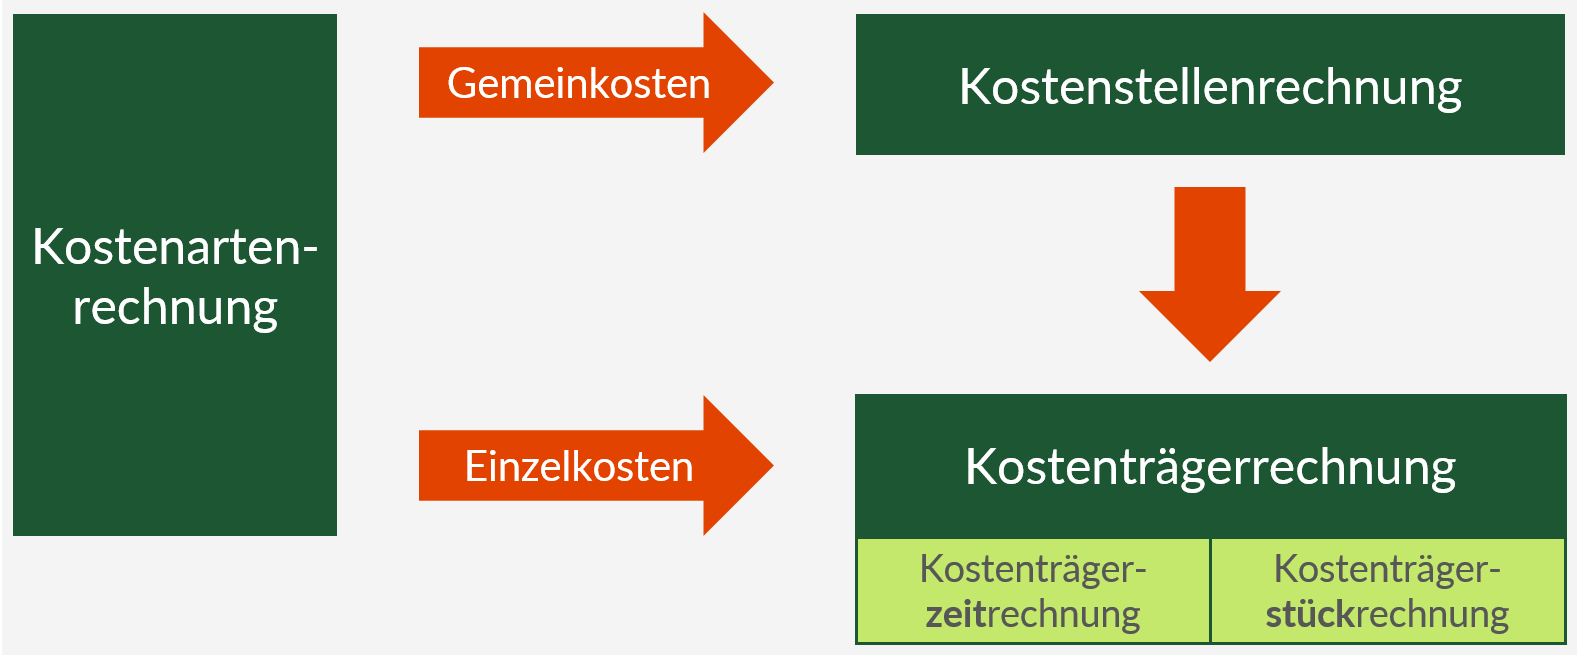
\includegraphics[keepaspectratio]{images/figure22.png}} \hfill{}

\caption{Abb. 2.2: Kostenrechnungsstufen im internen Rechnungswesen
(Trummer, o.J.). Quelle:
h\href{https://www.modu-learn.de/wordpress/wp-complete/uploads/2017/07/kostenanalyse-basis-neu.png}{ttps://www.modu-learn.de/wordpress/wp-complete/uploads/2017/07/kostenanalyse-basis-neu.png}}

\end{figure}%

Die~\emph{Kostenartenrechnung}~versucht, alle Kostenarten zu ermitteln,
, d. h. sie geht der Frage nach, welche Kosten insgesamt in der
Einrichtung anfallen. Dies sind z. B. Personalausgaben oder auch
Abschreibungen. In der~\emph{Kostenstellenrechnung}~gilt es zu
ermitteln, wo diese Kosten angefallen sind: in der Kindertagesgruppe, im
Einkauf, bei der Geschäftsleitung, in der Öffentlichkeitsarbeit oder an
sonstigen Stellen. Die~\emph{Kostenträgerrechnung}~beschäftigt sich mit
der Frage, wo die Kosten anfallen, also für welche Produkte und
Dienstleistungen. Da stellt sich die Frage, wie hoch die Kosten sind,
die im Rahmen einer Beratungsstunde, einer Betreuungsstunde oder ganz
allgemein im Rahmen eines Tagessatzes angefallen sind. Darunter lassen
sich alle Personalkosten fassen, also alle Sachkosten, die in
unterschiedlichen Kostenstellen angefallen sind. Sodann lässt sich
problemlos feststellen, wie „teuer'' eine Dienstleistung tatsächlich
ist.

\subsection{Phasen des Controllings}\label{phasen-des-controllings}

Im Controlling, wie vorangehend bereits ausgeführt, geht es um die
Aufgabe, klar zu planen und entsprechende Abweichungen frühzeitig
festzustellen, um daraus Maßnahmen abzuleiten. Hier sei ein Modell von
Bachmann ((Bachmann 2008)) angeführt, der sich mit den verschiedenen
Phasen des Controllings beschäftigt (vgl. \hyperref[figure23]{Abb.
2.3}).

\begin{figure}

\pandocbounded{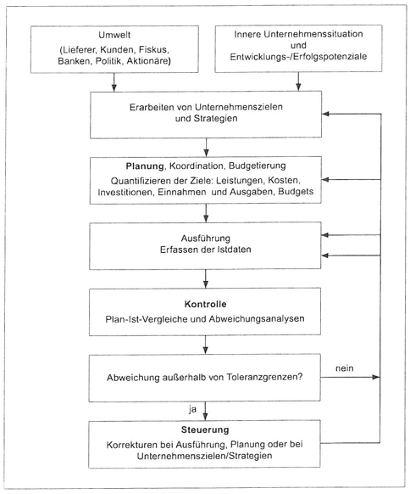
\includegraphics[keepaspectratio]{images/figure23.png}} \hfill{}

\caption{Abb. 2.3: Phasen des Controllings nach (Bachmann 2008, S. 9)}

\end{figure}%

Neben dem Controlling müssen am Anfang erstmal eine~\emph{Umweltanalyse
sowie unternehmensinterne Analysen}~durchgeführt werden, um
herauszufinden, mit welchen Stakeholdern überhaupt eine Verbindung
besteht. Es sind die Rahmenbedingungen der jeweiligen Situation zu
beschreiben. Anschließend wird daraus ganz allgemein die Zielstellung
für die Einrichtung herausgearbeitet, sodass dies zum Beispiel in
einem~\emph{strategischen Plan}~von Jahr zu Jahr erneuert werden kann.

Nach Festlegung der Zielstellungen geht es in der nächsten Phase um
die~\emph{Planung}~einer konkreten Wirtschaftsperiode. Dies kann bspw.
im Rahmen von Budgets oder mithilfe der Budgetierung getan werden, um
damit alle Kosten und Leistungen der Einrichtung geteilt oder nach den
Einrichtungsteilen gegliedert zu ermitteln.

Schließlich müssen im Laufe des Jahres die verschiedenen tatsächlich
angefallenen Kosten erfasst werden. Diese sind tabellarisch im Budget zu
erfassen. Mit diesem Wissen ausgestattet ist man in der Lage,
die~\emph{Kontrollmaßnahmen}~durchzuführen, ob sich bspw. Abweichungen
ergeben haben oder ob überhaupt Abweichungen entstanden sind.\\
\strut \\
Sofern~\emph{Abweichungen}~entstanden sind, muss überlegt werden, ob
diese vor dem Hintergrund definierter Toleranzgrenzen tolerierbar ist.
Wenn eine Kostenstelle leicht überzogen wurde, müssen nicht gleich die
härtesten Maßnahmen, wie z. B. ein Kostenstopp für alle zukünftigen
Anschaffungen ausgesprochen werden. Lohnsteigerungen im Umfang von 2 bis
4 \% sind beispielsweise etwas Normales. Dies kann sich durch
Tarifveränderungen oder eine Steigerung der Sozialabgaben ergeben haben.

Wenn allerdings die Toleranzgrenzen überschritten sind, dann müssen
entsprechende Veränderungsmaßnahmen eingeleitet werden. Dazu dient die
letzte Phase der~\emph{Steuerung}. Hier müssen Korrekturmaßnahmen
eingeleitet werden, damit die Ziele, die ursprünglich gesetzt worden
sind, auch erreicht werden können.

An der Seite sind verschiedene Pfeile erkennbar, die andeuten sollen,
dass hier verschiedene~\emph{Feedbackprozesse}~möglich sind. In der
ersten Phase widmet man sich kurzgesagt der~\emph{Planung}. Die zweite
Phase fragt danach, wie kontrolliert werden kann
und~\emph{Abweichungen}~ermittelt werden können. In der dritten Phase
beschäftigt man sich mit den
verschiedenen~\emph{Handlungsempfehlungen}~und Instrumenten, die
aufgetretenen Abweichungen wieder zu korrigieren.

\section{Personalmanagement}\label{personalmanagement}

Management ganz allgemein bedeutet: eine zielorientierte Gestaltung und
Steuerung von Organisationen. Beim Personalmanagement bzw. in der
Personalwirtschaft geht es darum, die Einrichtung durch Maßnahmen zu
gestalten, die darauf abzielen, einerseits neues Personal zu gewinnen,
das Personal zu verwalten bzw. zu erfassen und andererseits auch für die
Personalentwicklung der Mitarbeitenden aufzukommen (z.B. (Ribbeck 2020).
Das muss hinsichtlich wirtschaftlicher, sozialer und auch individueller
Zielsetzung geschehen. Es gibt ein umfangreiches Aufgabenpaket für das
Personalmanagement (vgl. \hyperref[figure24]{Abb. 2.4}).

\begin{figure}

\pandocbounded{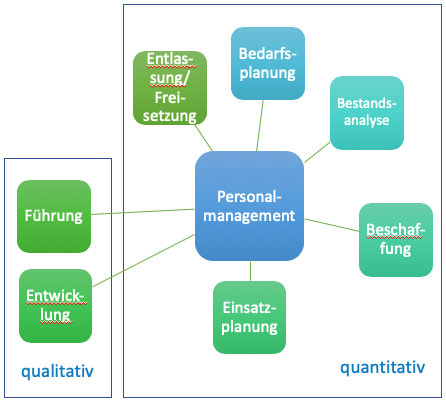
\includegraphics[keepaspectratio]{images/figure24.png}} \hfill{}

\caption{Abb. 2.4: Aufgabenfelder des Personalmanagements (in Anlehnung
an Hölzle 2006, S.18)}

\end{figure}%

Zunächst gibt es die Bedarfsplanung. Mit~\emph{Bedarfsplanung}~ist
gemeint, dass man sich Gedanken machen muss, wer mit welchen Kompetenzen
in welchen Betriebsteilen zukünftig eingeplant werden soll. Das
erfordert die regelmäßige Erfassung von Personalstatistiken und das
Sammeln von personenbezogenen Daten (\emph{Bedarfsanalyse}). Die
Beschaffung -- der Begriff kommt aus der Produktionswirtschaft -- meint
hier die Akquise von Personal. Das kann von außen geschehen, das kann
aber auch intern geschehen. Außen wäre beispielsweise die
Stellenanzeige, intern eine Umsetzung oder Veränderung von
Arbeitsverträgen.

Die~\emph{Einsatzplanung}~beschäftigt sich mit der Aufgabe, kurz- bzw.
mittelfristig Dienstpläne zu erstellen. Längerfristig ist die
Einsatzplanung zum Beispiel dazu wichtig, um Karrierewege planen zu
können.

Schließlich sind gelegentlich noch \emph{Entlassungen} und
\emph{Freisetzungen} durchzuführen. Für das Personalmanagement
gesprochen, handelt es sich bei Entlassungen um die Trennung von
Mitarbeitenden. Freisetzung ist ein Sammelbegriff dafür, dass es
alternative Maßnahmen gibt, die möglicherweise eine Entlassung
verhindern können oder vermeiden lassen, wie z. B. innerbetriebliche
Versetzungen, auch Umschulungen für eine andere Stelle, Kurzarbeit oder
auch Urlaub und Sonderurlaub.

Es gibt im Personalmanagement noch die Aufgabenbereiche
der~\emph{Führung}~und~\emph{Entwicklung}. Mit Führung ist gemeint, dass
jede Leitungskraft selbst reflektieren muss und entsprechendes Wissen,
Fähigkeiten und Erfahrungen besitzen muss, ein Team zu leiten, eine
Einrichtung zu leiten und Mitarbeitende zu motivieren. Sie muss auch
selbst in der Lage sein, das eigene Leitungshandeln zu hinterfragen.
Entwicklungsaufgaben ergeben sich durch die Personalentwicklung in den
Einrichtungen, d.~h. Kompetenzen müssen ständig weiterentwickelt und
durch geeignete Maßnahmen gewährleistet werden. Darunter fallen z. B.
Personalweiterbildungen.

Das Personalmanagement kann einerseits in
einen~\emph{quantitativen}~Teil (das sind die ersten fünf aufgeführten
Bereiche) und in einen~\emph{qualitativen}~Teil unterteilt werden (z.B.
Hölzle 2006).

\section{Organisationsentwicklung und
Change-Management}\label{organisationsentwicklung-und-change-management}

Zu diesem Funktionsbereich sei ein Modell der Organisationsentwicklung
bzw. des Change-Managements von Kurt Lewin angeführt. Dieser hat ein
Drei-Phasen-Modell entwickelt, welches mit der Metapher des Auftauens
und Einfrierens von Organisationsstrukturen argumentiert (vgl.
\hyperref[figure25]{Abb. 2.5}).

\begin{figure}

\pandocbounded{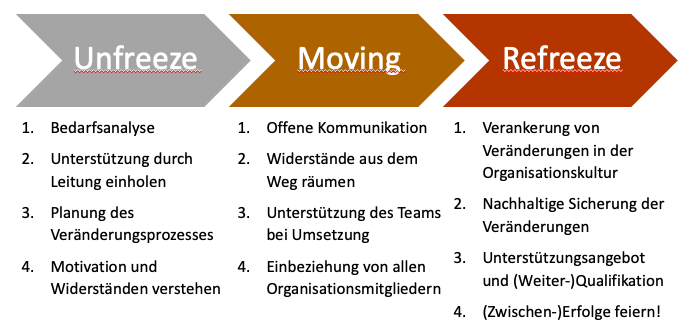
\includegraphics[keepaspectratio]{images/figure25.png}} \hfill{}

\caption{Abb. 2.5: Organisationsentwicklung und Change-Management nach
Kurt Lewins 3-Phasen-Modell (eigene Darstellung)}

\end{figure}%

In der ersten Phase, dem~\emph{Unfreezing}, geht es grundsätzlich darum,
den Bedarf und die Situation zu klären. Es muss ermittelt werden, was
verändert werden muss, wie dieser Prozess geplant werden kann, unter
welchen Umständen Mitarbeitende mitgenommen werden können und mit
welchen Widerständen ggf. gerechnet werden muss.

In der~\emph{Moving}-Phase geht es darum, offen zu kommunizieren, was
genau die Veränderung ist. Die Veränderungsprozesse müssen umgesetzt,
Widerstände behandelt und das Team regelmäßig einbezogen werden. Es sind
Fragestellungen und die dazugehörigen Lösungen zu entwickeln.
Letztendlich sollte regelmäßig über den aktuellen Stand in
Großgruppenveranstaltungen informiert werden.

In der~\emph{Refreezing}-Phase, dem Einfrieren, müssen die geänderten
Strukturen gefestigt werden. Es werden die neuen gefundenen Strukturen
und definierten Prozesse verankert. Das dient dazu, nachhaltig mit den
neuen Arbeitsstrukturen zu arbeiten und gegebenenfalls
Anpassungsqualifikationen durchzuführen. Wenn die Maßnahme erfolgreich
umgesetzt wurde, gilt es natürlich auch zum Schluss, den Erfolg zu
feiern.

\section{Sozio-Marketing}\label{sozio-marketing}

Schließlich gibt es noch den betriebswirtschaftlichen Funktionsbereich
des Marketings bzw. das~\emph{Sozio-Marketing}, also das Marketing
sozialer Einrichtungen.

\emph{Marketing}~ist zusammengefasst der Aufgabenbereich, der sich damit
beschäftigt, die jeweiligen Dienstleistungen und Produkte einerseits
hinsichtlich ihrer Qualität zu entwickeln und Werte zu schaffen sowie
andererseits zu kommunizieren sowie Kunden anzubieten und diese
Austauschbeziehung zu managen.

Nach Harald Christa (Christa 2010) ist~\emph{Sozio-Marketing}~„auf eine
konkrete Organisation der sozialen Arbeit bzw. der Wohlfahrtspflege
bezogen'', „umfasst weit mehr als rein kommunikationspolitische
Facetten'', „Anwendung der Denkweisen undInstrumente des Marketings in
und für soziale Organisationen'' (Christa 2010, S. 19, 24). Mithin
stellt sich die Aufgabe, die allgemeinen betriebswirtschaftlichen
Grundlagen des Marketings auf soziale Einrichtungen zu übersetzen.

Im Folgenden soll beispielhaft der \emph{Vier-Felder-Marketingmix}, ein
bekanntes Instrument des Marketings, vorgestellt werden. Dies ist dazu
geeignet, verschiedene Aufgaben bzw. Handlungsfelder des Marketings
zusammenzufassen, wobei unterschieden wird zwischen Leistungspolitik,
Preispolitik, Distributionspolitik und Kommunikationspolitik (vgl.
\hyperref[figure26]{Abb. 2.6}).

\begin{figure}

\pandocbounded{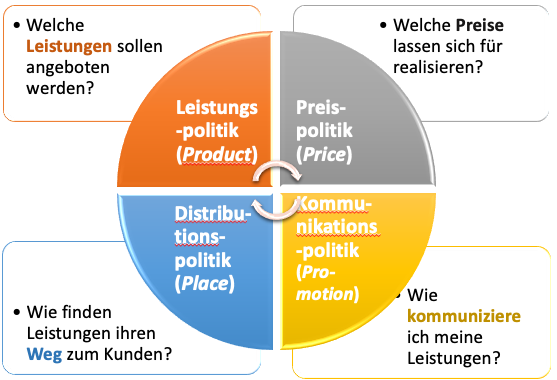
\includegraphics[keepaspectratio]{images/figure26.png}} \hfill{}

\caption{Abb. 2.6: Marketing-Mix (eigene Darstellung)}

\end{figure}%

In der~\emph{Leistungspolitik}~geht es um die Frage, welche Leistungen
überhaupt angeboten werden. Es muss ermittelt werden, wie die
marktgerechte Ausgestaltung der Leistung aussieht und welche Aussagen
sich von der Erhebung der Klient*innen- sowie Kundenbedarfe ergeben. Das
ist notwendig, um ermitteln zu können, ob die Qualität entsprechend gut
ist, sodass die Erwartungen der Kunden befriedigt werden. Des Weiteren
ist in Umwelt- oder Umfeldanalysen zu erforschen, wie sich das Produkt
bzw. die Dienstleistung von anderen unterscheidet. Eventuell ließe sich
eine Qualitäts- oder Kostenführerschaft übernehmen. Schließlich ist in
der Leistungspolitik auch eine „Unique selling proposition'' (USP) von
Bedeutung; ein Alleinstellungsmerkmal der Einrichtung muss
herausgearbeitet werden.

In der~\emph{Preispolitik}~geht es um die Frage, wie der Preis gestaltet
wird und wie sich Preise realisieren lassen. Darauf haben wir in der
Sozialwirtschaft weniger Einfluss, weil die Preise festgelegt sind, wenn
wir beispielsweise an die Leistungsentgelte denken, wobei diese Entgelte
im Regelfall feststehen. Nichtsdestotrotz müssen die Preise dahingehend
kalkuliert werden, wie z. B. durch eine Kostenanalyse soll ein Überblick
über die Kostenstruktur ermittelt werden. So muss ermittelt werden, wie
teuer eine Beratungsstunde oder ein Tagessatz ist. Wenn diese Berechnung
erfolgt ist, kann man in die Leistungsentgeltverhandlungen gehen und den
notwendigen Preis verlangen, damit alle Kosten der Einrichtung gedeckt
werden können. Es gibt ganz unterschiedliche Wege zur Preisfindung. Hier
wurde das Modell der Kostenorientierung vorgestellt. Man kann sich aber
auch bspw. bei der Kalkulation von Weiterbildungen an der Konkurrenz
orientieren. Man kann sich auch anhand der Nachfrage orientieren, also
dem Nutzer der jeweiligen Dienstleistungen. Darüber hinaus gibt es noch
das Target Costing, also die ziel- und nutzenorientierte Ermittlung von
Kosten bzw. Preisen. Die letztgenannten Verfahren sind eher im
Weiterbildungs- bzw. allgemein im Bildungsbereich passend.

Die~\emph{Distributionspolitik}~fragt danach, auf welchem Wege die
Leistungen zum Kunden gebracht werden. Es gibt sog. Absatzmittler wie z.
B. Schuldnerberatungen, die manchmal ein erster Anlaufpunkt für Menschen
in besonderen, finanziellen wie persönlichen Lebenslagen sind. Sie
können Menschen an andere Beratungen verweisen. Darüber hinaus gibt es
die Meinungsführer („Influencer''). Das sind diejenigen
meinungsbildenden Personen, die die Einrichtung kennen und
weiterempfehlen. Das können beispielsweise Selbsthilfegruppen, Elternrat
und Elterngruppen, aber auch andere Vereinigungen bzw.
Wohlfahrtsverbände sein, die auf unsere Einrichtung hinweisen. Die
Standortwahl ist ebenso ein Aspekt in Distributionspolitik. Es ist dabei
zu analysieren, wo sich die Einrichtung befindet: in einer Randlage oder
im Stadtzentrum. Davon hängt ab, welche Personen sie erreichen kann.
Schließlich sind die Öffnungszeiten sowie die Erreichbarkeit mit
öffentlichen Verkehrsmitteln entscheidend.

Den letzten großen Teil des Marketing-Mix stellt
die~\emph{Kommunikationspolitik}~dar. Hier geht es um die Frage, wie die
Leistungen kommuniziert werden können, sodass sie dann entweder die
gesamte Bevölkerung erreichen oder gezielt einzelne Gruppen ansprechen.
Es geht um die Erhöhung des Bekanntheitsgrades der Einrichtung in der
Öffentlichkeitsarbeit. Im Rahmen der Werbung müssen die
unterschiedlichen Kanäle und Medien gewählt werden: ob über Social
Media, über Werbung, über direkten Kontakt oder über eine Website.
Herausgearbeitet werden muss, mit welcher Botschaft man die Personen
erreicht, die man ansprechen will.

\section{Weitere Funktionsbereiche}\label{weitere-funktionsbereiche}

Abschließend ist ein Überblick über weitere Funktionsbereiche zu geben,
gewissermaßen die Balkone und das Dach des Hauses der BWL. Hierzu
erfolgt nur eine sehr sporadische Zusammenfassung in der folgenden
Abbildung. All diese Bereiche, die hier aufgeführt sind, haben eine
separate Veranstaltung im Laufe Ihres Studiums (vgl.
\hyperref[figure27]{Abb. 2.7}).

\begin{figure}

\pandocbounded{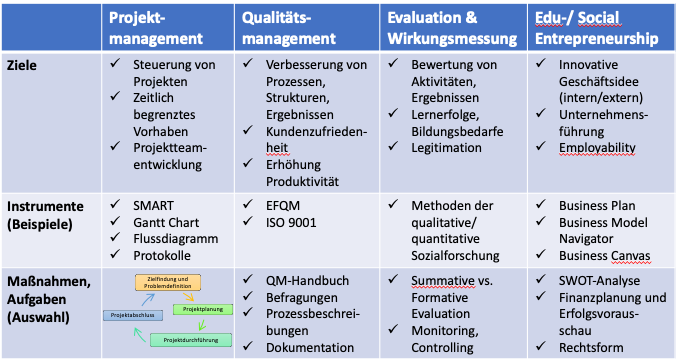
\includegraphics[keepaspectratio]{images/figure27.png}} \hfill{}

\caption{Abb. 2.7: Überblick weitere Bereich des Bildungsmanagements
(eigene Darstellung)}

\end{figure}%

Das~\emph{Projektmanagement}, darauf wurde bereits eingegangen, hat die
Aufgabe, Projekte zu steuern bzw. das Projektteam zu führen. Dabei
handelt es sich um befristete Maßnahmen. Am Anfang muss man sich
Gedanken über die Ziele zum Projekt machen. Es muss ein Plan entwickelt
werden, dieser umgesetzt sowie durchgeführt werden. Zum Schluss werden
die Ergebnisse veröffentlicht bzw. daraus ergibt sich möglicherweise ein
neues Thema, was in einem anderen Projekt umgesetzt werden kann. Die
smarte Zielformulierung kann hier als Instrument eingesetzt werden.
Ebenso können Charts dazu dienen, einen Projektplan zu entwickeln, aus
dem hervorgeht, zu welchem Zeitpunkt wann wer welche Tätigkeiten
übernimmt. Flussdiagramme sind hilfreich, um Prozesse zu beschreiben.
Zudem sind Protokolle von Meetings anzufertigen.

Das~\emph{Qualitätsmanagement}~hat die Aufgabe, Prozesse, Strukturen und
Ergebnisse regelmäßig zu überprüfen. Es bildet gewissermaßen einen
Garanten, um Standardisierung oder Professionalisierung zu ermöglichen.
In dessen Rahmen ist regelmäßig danach zu fragen, wie sich die
Kundenzufriedenheit darstellt und ob sich diese verändert hat. Umfassend
muss geprüft werden, wie die gesamte Einrichtung noch effektiver und
produktiver werden kann. Dazu gibt es verschiedene Modelle wie z. B. das
EFQM-Modell oder die DIN-ISO-Norm. Im Bereich der Sozial- und
Gesundheitswirtschaft gibt es noch zahlreiche andere Modelle und
Instrumente, die eingesetzt werden können. Im Qualitätsmanagement werden
verschiedene Maßnahmen festgelegt, Prozesse beschrieben und
dokumentiert, zudem sollte auch ein Qualitätsmanagement-Handbuch
entstehen.

Die~\emph{Evaluation bzw. Wirkungsmessung}~fragt danach, wie die
Aktivitäten und Ergebnisse, die sich im Rahmen der Tätigkeiten ergeben
haben, bewertet werden können. Zu ermitteln ist, was die Wirkungen sind,
die sich daraus ergeben und welche Effekte sich auf sozialer,
organisationaler und möglicherweise kommunaler sowie Sozialraumebene
ergeben. Sie dienen dazu, Lernerfolge, Bildungsbedarf und -veränderung
sowie Kompetenzentwicklungen abzubilden. In diesem Bereich nutzt man
Methoden der qualitativen und quantitativen Sozialforschung, um genau
diese Ergebnisbewertungen vorzunehmen. Die Evaluation hat das Ziel,
herauszufinden, wie die Ergebnisse der jeweiligen Maßnahme gegenüber
ihren Zielen zu einer wirkungsvollen Veränderung geführt haben. Die
formative Evaluation beschäftigt sich mit der schrittweisen und
begleitenden Evaluation und versucht, im Prozess eines Programms, einer
Maßnahme oder eines Projektes entsprechend durch Feedback und
Reflexionsmöglichkeiten auf den Verlauf von Monitoring- und
Controlling-Maßnahmen Einfluss zu nehmen. Die summative Evaluation
ermittelt die Wirkung nach Abschluss der Maßnahme.

Die~\emph{Evaluation bzw. Wirkungsmessung}~fragt danach, wie die
Aktivitäten und Ergebnisse, die sich im Rahmen der Tätigkeiten ergeben
haben, bewertet werden können. Zu ermitteln ist, was die Wirkungen sind,
die sich daraus ergeben und welche Effekte sich auf sozialer,
organisationaler und möglicherweise kommunaler sowie Sozialraumebene
ergeben. Sie dienen dazu, Lernerfolge, Bildungsbedarf und -veränderung
sowie Kompetenzentwicklungen abzubilden. In diesem Bereich nutzt man
Methoden der qualitativen und quantitativen Sozialforschung, um genau
diese Ergebnisbewertungen vorzunehmen. Die Evaluation hat das Ziel,
herauszufinden, wie die Ergebnisse der jeweiligen Maßnahme gegenüber
ihren Zielen zu einer wirkungsvollen Veränderung geführt haben. Die
formative Evaluation beschäftigt sich mit der schrittweisen und
begleitenden Evaluation und versucht, im Prozess eines Programms, einer
Maßnahme oder eines Projektes entsprechend durch Feedback und
Reflexionsmöglichkeiten auf den Verlauf von Monitoring- und
Controlling-Maßnahmen Einfluss zu nehmen. Die summative Evaluation
ermittelt die Wirkung nach Abschluss der Maßnahme.

In dieser Grundlagenveranstaltung wurden ausgewählte Funktionsbereiche
dargestellt, die in jeder Einrichtung eine Rolle spielen, unabhängig
davon, ob es sich um eine soziale oder um eine erwerbswirtschaftliche
Einrichtung im weitesten Sinne handelt.

\cleardoublepage
\phantomsection
\addcontentsline{toc}{part}{Appendices}
\appendix

\chapter{Literaturverzeichnis}\label{literaturverzeichnis}

\phantomsection\label{refs}
\begin{CSLReferences}{1}{0}
\bibitem[\citeproctext]{ref-Arnold2022b}
Arnold, Maik. 2022a. {``Hybrid Function of Social Work Management
Education.''} figshare.
\url{https://doi.org/10.6084/M9.FIGSHARE.20079650.V1}.

\bibitem[\citeproctext]{ref-Arnold2022a}
---------. 2022b. {``{Social Work Management Subject Map},''} June.
\url{https://doi.org/10.6084/m9.figshare.20151839.v1}.

\bibitem[\citeproctext]{ref-arnold2019Finanzbuchhaltunga}
---------. 2024. {``Finanzbuchhaltung.''} In \emph{Das große Handbuch
Organisation und Verwaltung in der Kita}, edited by Harald Christa, 2nd
ed., 243--64. Köln: Carl Link.

\bibitem[\citeproctext]{ref-bachmann2008}
Bachmann, P. 2008. \emph{Grundlagen Des Controlling in Sozialen
Organisationen}. 2. Aufl. Brandenburg: Hochschulverbund Distance
Learning (HDL Nr. 2-020-2601).

\bibitem[\citeproctext]{ref-Beck2013}
Beck, Reinhilde, Klaus Grunwald, Klaus Schellberg, Gotthart Schwarz,
Wolf Rainer Wendt, and Armin Wöhrle. 2013. {``Kapitel 1
Sozialwirtschaft.''} In \emph{Grundlagen Des Managements in Der
Sozialwirtschaft}, 11--34. Nomos Verlagsgesellschaft mbH \& Co. KG.

\bibitem[\citeproctext]{ref-Boessenecker2014}
Boeßenecker, Karl-Heinz, and Andreas Markert. 2014. \emph{Studienführer
Sozialmanagement}. Nomos. \url{https://doi.org/10.5771/9783845250915}.

\bibitem[\citeproctext]{ref-Brinkmann2010}
Brinkmann, Volker. 2010. \emph{Sozialwirtschaft}. Gabler.
\url{https://doi.org/10.1007/978-3-8349-8935-2}.

\bibitem[\citeproctext]{ref-Bundesagentur2014beschaeftigte}
Bundesagentur für Arbeit Berichte. 2014/2020. {``Beschäftigte Nach
Wirtschaftszweigen (WZ 2008) (Monatszahlen).''}
\url{https://statistik.arbeitsagentur.de/Statistikdaten/Detail/202007/iiia6/beschaeftigung-sozbe-monatsheft-wz/monatsheft-wz-d-0-202007-pdf.pdf?__blob=publicationFile&v=1}
(2020),
\url{https://statistik.arbeitsagentur.de/Statistikdaten/Detail/201409/iiia6/beschaeftigung-sozbe-monatsheft-wz/monatsheft-wz-d-0-201409-pdf.pdf?__blob=publicationFile&v=1}
(2014).

\bibitem[\citeproctext]{ref-Christa2010}
Christa, Harald. 2010. \emph{Grundwissen Sozio-Marketing}. VS Verlag für
Sozialwissenschaften. \url{https://doi.org/10.1007/978-3-531-92438-0}.

\bibitem[\citeproctext]{ref-Europeancommission2015social}
European Commission. 2015. {``The Social Business Initiative of the
European Commission.''}
\url{http://ec.europa.eu/DocsRoom/documents/14583}.

\bibitem[\citeproctext]{ref-Evers2010}
Evers, Adalbert, and Benjamin Ewert. 2010. {``Hybride Organisationen Im
Bereich Sozialer Dienste. Ein Konzept, Sein Hintergrund Und Seine
Implikationen.''} In \emph{Soziale Personenbezogene
Dienstleistungsorganisationen}, 103--28. VS Verlag für
Sozialwissenschaften. \url{https://doi.org/10.1007/978-3-531-92474-8_4}.

\bibitem[\citeproctext]{ref-helmig2019nonprofit}
Helmig, B. 2019. {``Nonprofit-Organisation (NPO).''} In \emph{Gabler
Wirtschaftslexikon}.
\url{https://wirtschaftslexikon.gabler.de/definition/nonprofit-organisation-npo-39562}.

\bibitem[\citeproctext]{ref-holzle2006}
Hölzle, C. 2006. \emph{Personalmanagement in Einrichtungen Der Sozialen
Arbeit: Grundlagen Und Instrumente}. Weinheim, München: Juventa.

\bibitem[\citeproctext]{ref-IDW2004wohlfahrtsverbaende}
Institut der Deutschen Wirtschaft Köln, ed. 2004.
\emph{Wohlfahrtsverbände in Deutschland: Auf Den Schultern Der
Schwachen}. Dt. Instituts-Verlag.
\url{https://www.yumpu.com/de/document/view/7199735/auf-den-schultern-der-schwachen}.

\bibitem[\citeproctext]{ref-Karmann2011gutachten}
Karmann, A., A. Werblow, B. Karmann, and A. Jurack. 2011. {``Gutachten
Zur Sozialwirtschaft in Sachsen Unter Besonderer Berücksichtigung Der
Freien Wohlfahrtspflege.''} Liga der Freien Wohlfahrt Sachsen.
\url{https://tu-dresden.de/bu/wirtschaft/wwsprofecon/ressourcen/dateien/publikationen/Sozialwirtschaft_2011.pdf?lang=de}.

\bibitem[\citeproctext]{ref-Klatetzki2010}
Klatetzki, Thomas. 2010. {``Zur Einführung: Soziale Personenbezogene
Dienstleistungsorganisation Als Typus.''} In \emph{Soziale
Personenbezogene Dienstleistungsorganisationen}, 7--24. VS Verlag für
Sozialwissenschaften. \url{https://doi.org/10.1007/978-3-531-92474-8_1}.

\bibitem[\citeproctext]{ref-Mross2017}
Mroß, Michael. 2017. {``Leistungsentgelt in Der Sozialwirtschaft.''}
\emph{Blätter Der Wohlfahrtspflege} 164 (6): 225--27.
\url{https://doi.org/10.5771/0340-8574-2017-6-225}.

\bibitem[\citeproctext]{ref-Ribbeck2020-vk}
Ribbeck, Jochen. 2020. \emph{Personalmanagement in Sozialunternehmen}.
WALHALLA Fachverlag.

\bibitem[\citeproctext]{ref-Ritter-Mamczek2016}
Ritter-Mamczek, Bettina. 2016. \emph{Stoff Reduzieren}. Kompetent
Lehren. Stuttgart, Germany: UTB.

\bibitem[\citeproctext]{ref-Schedler2013multirationales}
Schedler, Kuno, and Johannes Rüegg-Stürm. 2013. \emph{Multirationales
Management: Der Erfolgreiche Umgang Mit Widerspr{ü}chlichen
Anforderungen an Die Organisation}. Haupt.

\bibitem[\citeproctext]{ref-Schwarz1986management}
Schwarz, P. 1986. \emph{Management in Nonprofit-Organisationen:
{Ö}ffentliche Verwaltungen Und Betriebe, Verb{ä}nde, Vereine, Parteien,
Kirchen, Sozialwerke}. Schweizer Volksbank.

\bibitem[\citeproctext]{ref-Whoerle2007}
Wöhrle, Armin. 2007. {``Synergielösungen Für Sozialräume.''}
\emph{Blätter Der Wohlfahrtspflege} 154 (4): 153--55.
\url{https://doi.org/10.5771/0340-8574-2007-4-153}.

\bibitem[\citeproctext]{ref-Wohrle2017}
---------. 2017. {``25 Jahre Sozialmanagement -- Ein Kritischer
r{ü}ckblick.''} In \emph{Gegenwart Und Zukunft Des Sozialmanagements Und
Der Sozialwirtschaft}, 7--34. Wiesbaden: Springer Fachmedien Wiesbaden.

\end{CSLReferences}


\backmatter


\end{document}
